%File: anonymous-submission-latex-2025.tex
\documentclass[letterpaper]{article} % DO NOT CHANGE THIS
\usepackage[submission]{aaai25}  % DO NOT CHANGE THIS
\usepackage{times}  % DO NOT CHANGE THIS
\usepackage{helvet}  % DO NOT CHANGE THIS
\usepackage{courier}  % DO NOT CHANGE THIS
\usepackage[hyphens]{url}  % DO NOT CHANGE THIS
\usepackage{graphicx} % DO NOT CHANGE THIS
\urlstyle{rm} % DO NOT CHANGE THIS
\def\UrlFont{\rm}  % DO NOT CHANGE THIS
\usepackage{natbib}  % DO NOT CHANGE THIS AND DO NOT ADD ANY OPTIONS TO IT
\usepackage{caption} % DO NOT CHANGE THIS AND DO NOT ADD ANY OPTIONS TO IT
\frenchspacing  % DO NOT CHANGE THIS
\setlength{\pdfpagewidth}{8.5in} % DO NOT CHANGE THIS
\setlength{\pdfpageheight}{11in} % DO NOT CHANGE THIS
%
% These are recommended to typeset algorithms but not required. See the subsubsection on algorithms. Remove them if you don't have algorithms in your paper.
\usepackage{algorithm}
\usepackage{algorithmic}

%
% These are are recommended to typeset listings but not required. See the subsubsection on listing. Remove this block if you don't have listings in your paper.
\usepackage{newfloat}
\usepackage{listings}
\DeclareCaptionStyle{ruled}{labelfont=normalfont,labelsep=colon,strut=off} % DO NOT CHANGE THIS
\lstset{%
	basicstyle={\footnotesize\ttfamily},% footnotesize acceptable for monospace
	numbers=left,numberstyle=\footnotesize,xleftmargin=2em,% show line numbers, remove this entire line if you don't want the numbers.
	aboveskip=0pt,belowskip=0pt,%
	showstringspaces=false,tabsize=2,breaklines=true}
\floatstyle{ruled}
\newfloat{listing}{tb}{lst}{}
\floatname{listing}{Listing}
%
% Keep the \pdfinfo as shown here. There's no need
% for you to add the /Title and /Author tags.
\pdfinfo{
/TemplateVersion (2025.1)
}

\usepackage{amsmath}
\usepackage{array}
\usepackage{multirow}
\usepackage{booktabs}
\usepackage{diagbox}
\usepackage[table]{xcolor}
\usepackage{hhline}

% DISALLOWED PACKAGES
% \usepackage{authblk} -- This package is specifically forbidden
% \usepackage{balance} -- This package is specifically forbidden
% \usepackage{color (if used in text)
% \usepackage{CJK} -- This package is specifically forbidden
% \usepackage{float} -- This package is specifically forbidden
% \usepackage{flushend} -- This package is specifically forbidden
% \usepackage{fontenc} -- This package is specifically forbidden
% \usepackage{fullpage} -- This package is specifically forbidden
% \usepackage{geometry} -- This package is specifically forbidden
% \usepackage{grffile} -- This package is specifically forbidden
% \usepackage{hyperref} -- This package is specifically forbidden
% \usepackage{navigator} -- This package is specifically forbidden
% (or any other package that embeds links such as navigator or hyperref)
% \indentfirst} -- This package is specifically forbidden
% \layout} -- This package is specifically forbidden
% \multicol} -- This package is specifically forbidden
% \nameref} -- This package is specifically forbidden
% \usepackage{savetrees} -- This package is specifically forbidden
% \usepackage{setspace} -- This package is specifically forbidden
% \usepackage{stfloats} -- This package is specifically forbidden
% \usepackage{tabu} -- This package is specifically forbidden
% \usepackage{titlesec} -- This package is specifically forbidden
% \usepackage{tocbibind} -- This package is specifically forbidden
% \usepackage{ulem} -- This package is specifically forbidden
% \usepackage{wrapfig} -- This package is specifically forbidden
% DISALLOWED COMMANDS
% \nocopyright -- Your paper will not be published if you use this command
% \addtolength -- This command may not be used
% \balance -- This command may not be used
% \baselinestretch -- Your paper will not be published if you use this command
% \clearpage -- No page breaks of any kind may be used for the final version of your paper
% \columnsep -- This command may not be used
% \newpage -- No page breaks of any kind may be used for the final version of your paper
% \pagebreak -- No page breaks of any kind may be used for the final version of your paperr
% \pagestyle -- This command may not be used
% \tiny -- This is not an acceptable font size.
% \vspace{- -- No negative value may be used in proximity of a caption, figure, table, section, subsection, subsubsection, or reference
% \vskip{- -- No negative value may be used to alter spacing above or below a caption, figure, table, section, subsection, subsubsection, or reference

\setcounter{secnumdepth}{0} %May be changed to 1 or 2 if section numbers are desired.

% The file aaai25.sty is the style file for AAAI Press
% proceedings, working notes, and technical reports.
%

% Title

% Your title must be in mixed case, not sentence case.
% That means all verbs (including short verbs like be, is, using,and go),
% nouns, adverbs, adjectives should be capitalized, including both words in hyphenated terms, while
% articles, conjunctions, and prepositions are lower case unless they
% directly follow a colon or long dash
\title{From Persona to Person: Enhancing the Naturalness with Multiple Discourse Relations Graph Learning in Personalized Dialogue Generation}
\author{
    %Authors
    % All authors must be in the same font size and format.
    Chih-Hao Hsu, \\
    Hung-Yu Kao
}
\affiliations{
    %Afiliations
    \textsuperscript{\rm 1}Association for the Advancement of Artificial Intelligence\\
    % If you have multiple authors and multiple affiliations
    % use superscripts in text and roman font to identify them.
    % For example,

    % Sunil Issar\textsuperscript{\rm 2},
    % J. Scott Penberthy\textsuperscript{\rm 3},
    % George Ferguson\textsuperscript{\rm 4},
    % Hans Guesgen\textsuperscript{\rm 5}
    % Note that the comma should be placed after the superscript

    1101 Pennsylvania Ave, NW Suite 300\\
    Washington, DC 20004 USA\\
    % email address must be in roman text type, not monospace or sans serif
    proceedings-questions@aaai.org
%
% See more examples next
}

%Example, Single Author, ->> remove \iffalse,\fi and place them surrounding AAAI title to use it
\iffalse
\title{My Publication Title --- Single Author}
\author {
    Author Name
}
\affiliations{
    Affiliation\\
    Affiliation Line 2\\
    name@example.com
}
\fi

\iffalse
%Example, Multiple Authors, ->> remove \iffalse,\fi and place them surrounding AAAI title to use it
\title{My Publication Title --- Multiple Authors}
\author {
    % Authors
    First Author Name\textsuperscript{\rm 1},
    Second Author Name\textsuperscript{\rm 2},
    Third Author Name\textsuperscript{\rm 1}
}
\affiliations {
    % Affiliations
    \textsuperscript{\rm 1}Affiliation 1\\
    \textsuperscript{\rm 2}Affiliation 2\\
    firstAuthor@affiliation1.com, secondAuthor@affilation2.com, thirdAuthor@affiliation1.com
}
\fi


% REMOVE THIS: bibentry
% This is only needed to show inline citations in the guidelines document. You should not need it and can safely delete it.
\usepackage{bibentry}
% END REMOVE bibentry

\begin{document}

\maketitle

\begin{abstract}
In dialogue generation, the naturalness of responses is key for effective human-machine interaction, significantly enhancing user experience. Personalized response generation poses even greater challenges, as the responses must be coherent and consistent with the user's personal traits or persona descriptions. In this study, we propose a novel method named \textbf{MUDI} (\textbf{Mu}ltiple \textbf{Di}scourse Relations Graph Learning) aimed at effectively modeling and integrating discourse relations and persona information within the context of personalized dialogue generation. We initially utilize Large Language Models to assist in annotating discourse relations and to transform dialogue data into structured dialogue graphs. We employ our newly proposed DialogueGAT as the graph encoder, which captures implicit discourse relations within this structure. Persona descriptions are also encoded into completed persona graphs, facilitating the capture of semantic relationships between persona elements. An Attention-Based Feature Fusion method integrates data from both graphs, creating a personalized, coherence-aware dialogue representation. In the personalized response generation phase, a Prompt-based mechanism and a Coherence-Aware Attention strategy are implemented to enhance the decoder's consideration of discourse relations. Our experiments and case studies demonstrate significant improvements in the quality of personalized responses, making them more coherent, aligned with persona, and natural, thus resembling human-like dialogue exchanges.
\end{abstract}

% Uncomment the following to link to your code, datasets, an extended version or similar.
%
% \begin{links}
%     \link{Code}{https://aaai.org/example/code}
%     \link{Datasets}{https://aaai.org/example/datasets}
%     \link{Extended version}{https://aaai.org/example/extended-version}
% \end{links}

\begin{figure}[ht]
    \centering
    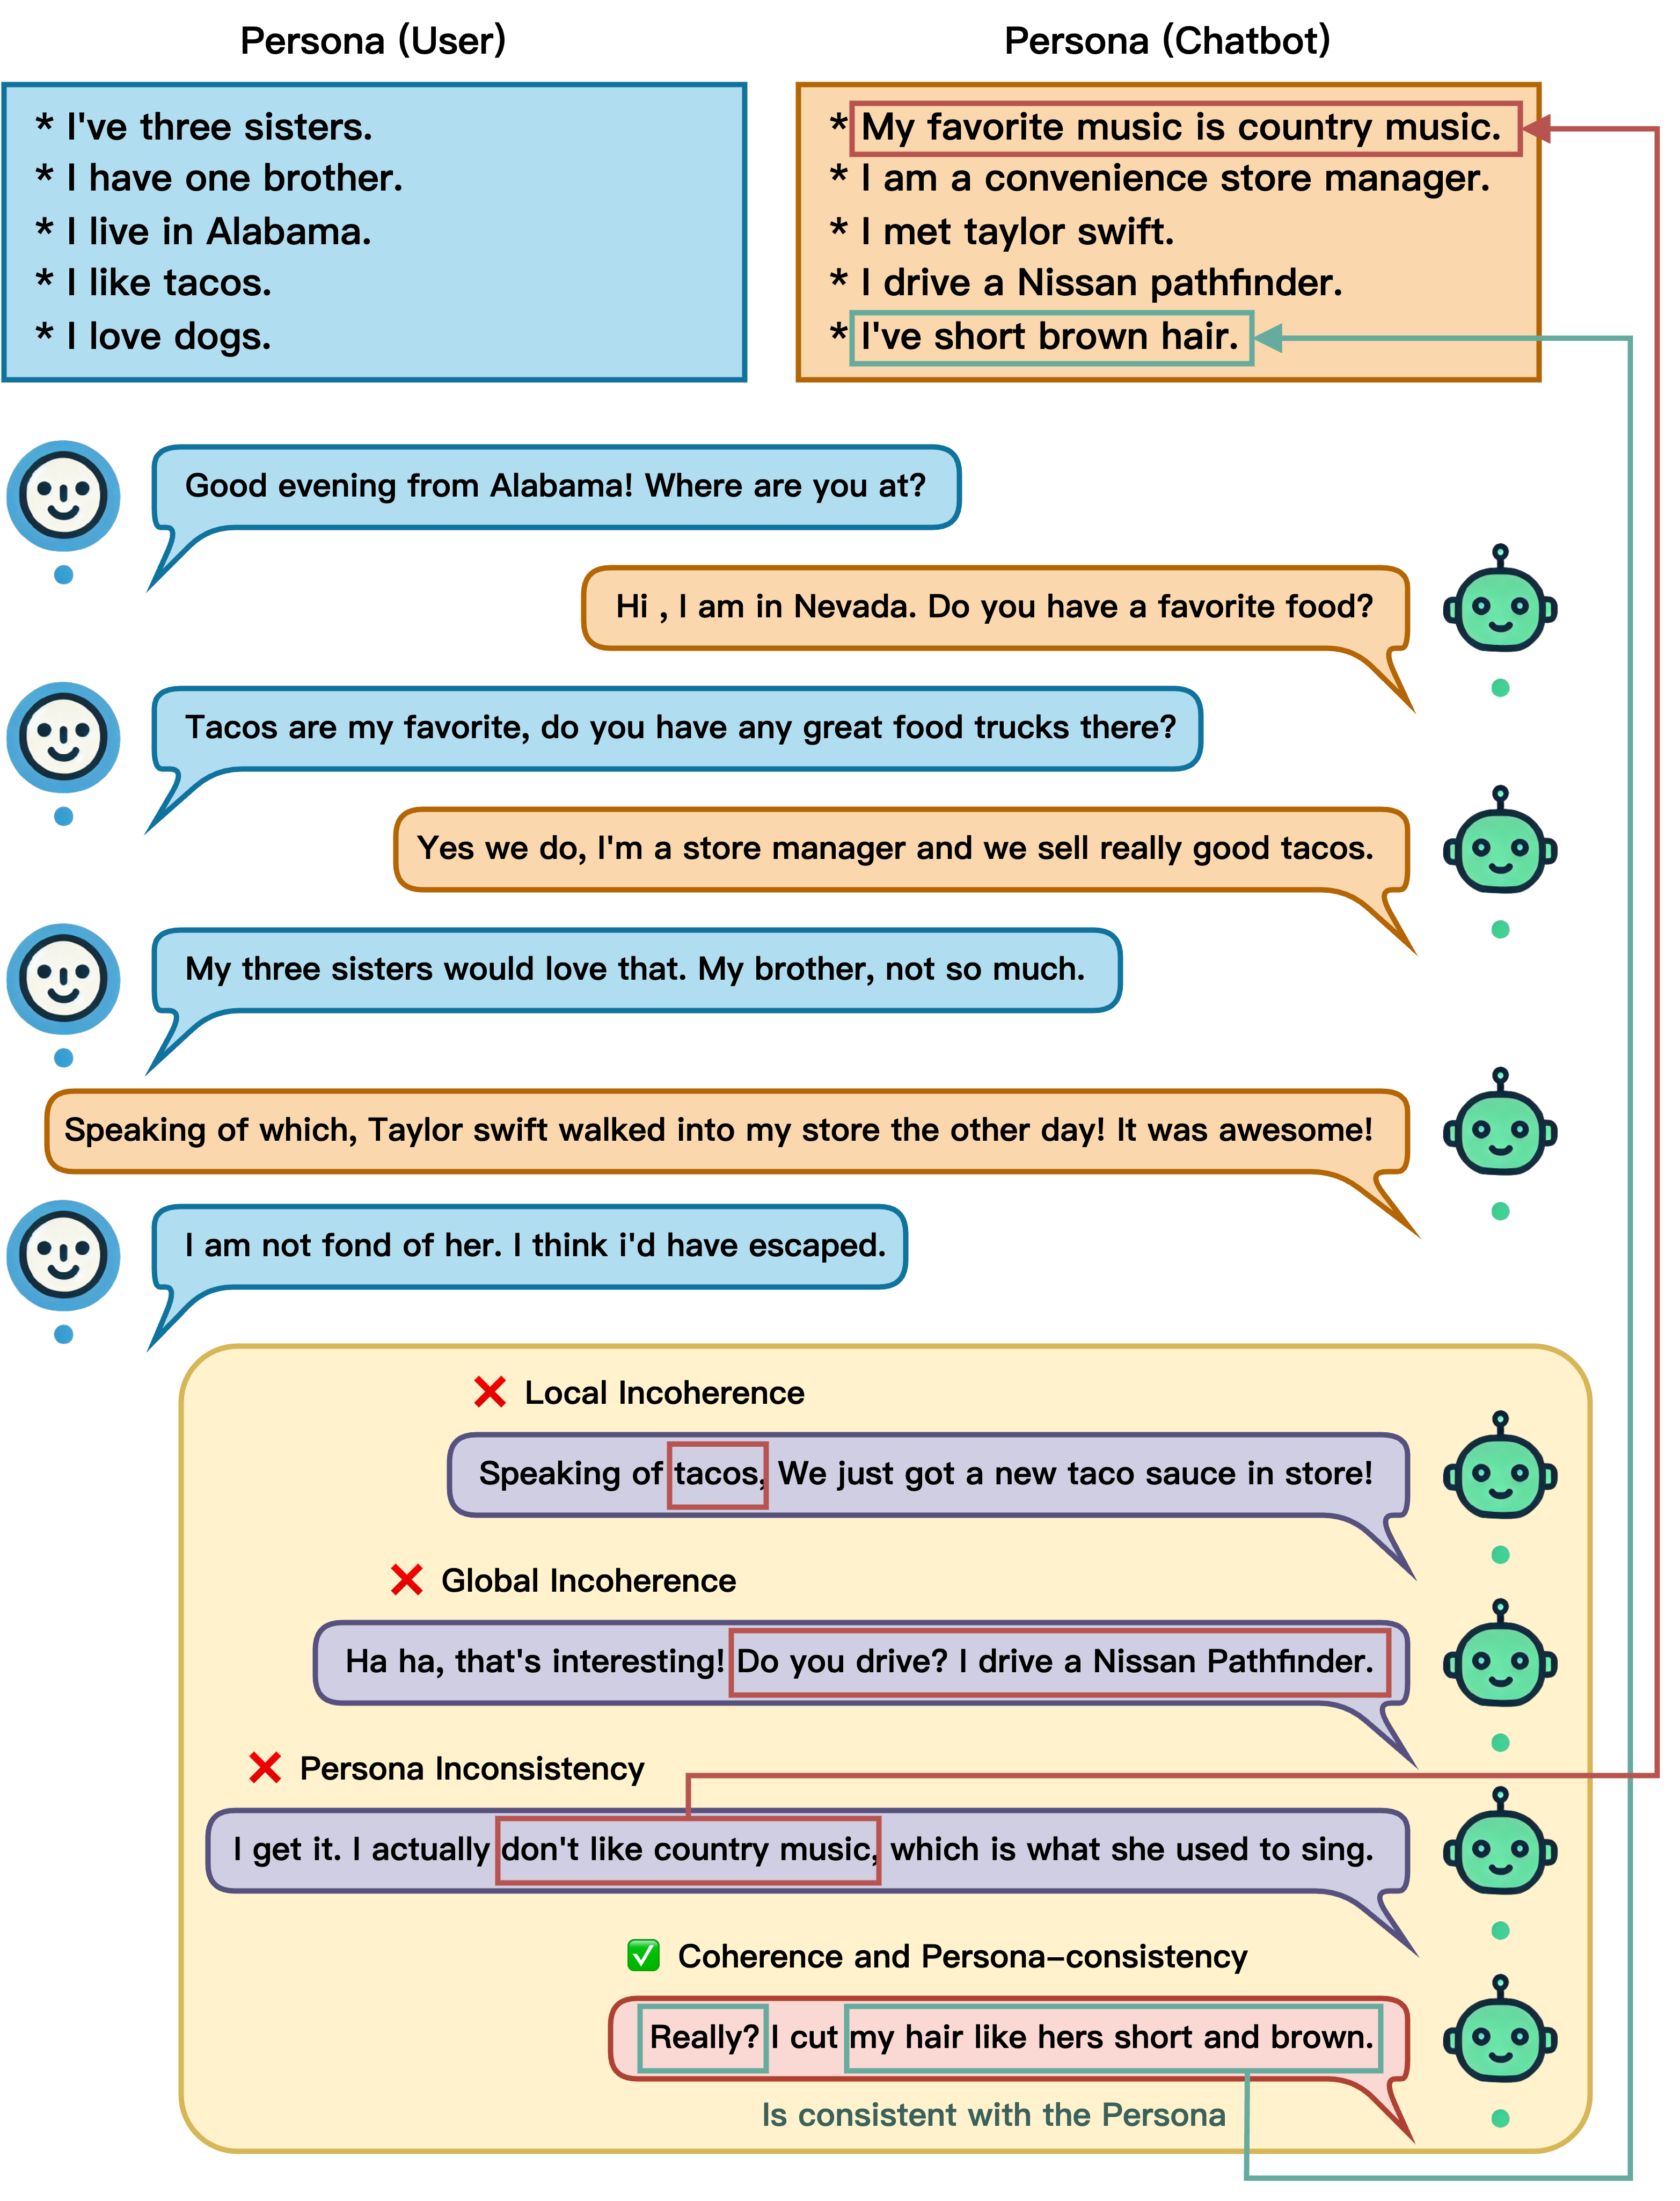
\includegraphics[width=0.32\textwidth]{./images/intro_pdg.png}
    \caption{Example of Incoherence and Persona Inconsistency issue in Personalized Dialogue Generation. This figure highlights the challenges in maintaining coherence and persona consistency in personalized dialogue system.}
    \label{fig:intro_pdg}
\end{figure}

\section{Introduction}
% Dialogue Generation is a foundational technology for dialogue systems, primarily focusing on the task of Next Utterance Generation, also known as Next Response Generation. In multi-turn dialogue scenarios, the conversational agent's objective is to analyze the context of the multi-turn dialogue and the current query to produce a following appropriate response. A significant drawback of traditional dialogue systems is their limited ability to personalize responses based on specific user characteristics or preferences. This limitation often results in generic and less engaging interactions that fail to meet individual user needs effectively \cite{jiang-de-rijke-2018-sequence}. Previous works \cite{song-etal-2020-generating, warren-2006-features} defined this problem as the naturalness issue of the Dialogue System. One effective solution to enhance the naturalness of dialogue systems is to integrate personality into the agents, referred to as "persona". Typically, a persona comprises several sentences describing the interlocutor's facts or background. This information is crucial for building a trustworthy and confident dialogue system. By endowing chatbot agents with human-like traits, the interactions become more realistic. Given these benefits, Personalized Dialogue Generation has emerged as a hot research topic in recent years, focusing on improving user engagement and satisfaction in dialogue systems.


% In recent years, there has been a surge of interest in personalized dialogue generation methods, spurred mainly by the release of publicly available large-scale datasets such as those introduced by Zhang et al. \cite{zhang-etal-2018-personalizing} and Dinan et al. \cite{dinan-etal-2019-convai2}. These datasets have significantly advanced efforts to enhance persona consistency and context understanding between generated responses and dialogue. For example, Liu et al. \cite{liu-etal-2020-impress} have concentrated on improving dialogue system consistency through more sophisticated modeling of interlocutor understanding. Song et al. \cite{song-etal-2021-bob} tackled persona-based dialogue generation by dividing it into two separate tasks: response generation and consistency understanding. They utilized unlikelihood training techniques to reduce the production of contradictory dialogue responses. Furthermore, Bao et al. \cite{bao-etal-2020-plato,bao-etal-2021-plato} employed latent variables to model response intentions and applied a response selection task to ensure that the generated responses align with both the dialogue context and background knowledge, such as persona information. Additionally, Huang et al. \cite{huang-etal-2023-paa} proposed a persona-adaptive attention that balances and regularizes the input information from persona and context, improving the consistent understanding of generated responses by persona and context.

% Despite these advances, significant challenges persist in enhancing engagement, response coherence, and persona consistency in dialogue systems. These challenges are primarily twofold. Firstly, many existing methods rely on sophisticated structures or external natural language inference (NLI) datasets to learn persona consistency. This approach, while effective, can sometimes lead the model to overly prioritize persona information at the expense of neglecting the broader dialogue context. Secondly, many dialogue-generating models fail to adequately consider the importance of discourse relations. They often neglect coherence, assuming that fluency alone can measure a dialogue's coherence. Discourse coherence, which focuses on how utterances are interconnected and the overall organization of dialogue to effectively convey information, is essential for effective conversation. Discourse coherence can be divided into local and global coherence. Local coherence refers to the logical connections between adjacent sentences, ensuring that they relate to each other and form a coherent sequence. Global coherence, on the other hand, extends beyond immediate sentence pairs to encompass higher-level relationships across the entire dialogue. This macro-linguistic capability allows conversational agents to maintain topic consistency and effectively convey meaning throughout an interaction. Poor global coherence can significantly impair the user's understanding of the discourse as a cohesive whole. As illustrated in Figure \ref{fig:intro_pdg}, the dialogue demonstrates various common issues encountered in personalized dialogue systems, including local and global incoherence as well as persona inconsistency. For example, consider the response "Speaking of tacos, we just got a new taco sauce in store!" This might seem appropriate and consistent with the persona in response to a query. However, this response could be incoherent within the broader context of the conversation. Additionally, the response "Ha ha, that's interesting! Do you drive? I drive a Nissan Pathfinder." is coherent with the query, but it introduces a strong and abrupt topic transition from the dialogue history. Furthermore, the remark "I get it. I actually don't like country music, which is what she used to sing." is not consistent with the persona, although it follows the conversation topic.

% In personalized dialogue generation, ensuring that the generated responses are consistent with the persona and coherent with the context of the dialogue is challenging. This is largely because inherent trade-offs exist between maintaining persona consistency and achieving discourse coherence. Few studies have successfully addressed the challenge of maintaining persona consistency while ensuring the generated responses' coherence. Moreover, the previous studies often omit explicit evaluations of Coherence, assuming that Fluency can also measure the coherence of dialogues. However, this approach does not directly account for the coherence of generated responses with the context and query, an aspect often presumed to be covered by fluency. To address these challenges, this study introduces a novel approach utilizing graph learning to retain both local and global coherence information in dialogues. Additionally, We leverage prompt learning and attention mechanisms to use discourse relations as signals for conditional response generation. Our proposed approach could guide the model to generate responses that are both coherent with the context and consistent with the persona, effectively enhancing the naturalness of the personalized dialogue generation.

Dialogue Generation is a foundational technology for dialogue systems, primarily focusing on the task of Next Utterance Generation, also known as Next Response Generation. In multi-turn dialogue scenarios, the conversational agent's objective is to analyze the context of the multi-turn dialogue and the current query to produce a following appropriate response. A significant drawback of traditional dialogue systems is their limited ability to personalize responses based on specific user characteristics or preferences. This limitation often results in generic and less engaging interactions that fail to meet individual user needs effectively \cite{jiang-de-rijke-2018-sequence}. Previous works \cite{song-etal-2020-generating, warren-2006-features} defined this problem as the naturalness issue of the Dialogue System. One effective solution to enhance the naturalness of dialogue systems is to integrate personality into the agents, referred to as "persona". Typically, a persona comprises several sentences describing the interlocutor's facts or background. This information is crucial for building a trustworthy and confident dialogue system. By endowing chatbot agents with human-like traits, the interactions become more realistic. Given these benefits, Personalized Dialogue Generation has emerged as a prominent research topic in recent years, focusing on improving user engagement and satisfaction within dialogue systems. This surge in interest is largely driven by the availability of large-scale personalized dialogue datasets, such as those from Zhang et al. \cite{zhang-etal-2018-personalizing} and Dinan et al. \cite{dinan-etal-2019-convai2}. These datasets have significantly advanced efforts to enhance persona consistency and context understanding in generated responses. Innovative methods, including Liu et al. \cite{liu-etal-2020-impress} have concentrated on improving dialogue system consistency through more complex modeling of interlocutor understanding. Song et al. \cite{song-etal-2021-bob} tackled persona-based dialogue generation by dividing it into two separate tasks: response generation and consistency understanding. They utilized unlikelihood training techniques to reduce the production of contradictory dialogue responses. Furthermore, Huang et al. \cite{huang-etal-2023-paa} proposed a persona-adaptive attention that balances and regularizes the input information from persona and context, improving the consistent understanding of generated responses by persona and context.

% persona-adaptive attention and unlikelihood training techniques, have been developed to align responses with both persona and context, effectively addressing challenges in persona consistency and coherence \cite{song-etal-2021-bob,huang-etal-2023-paa}.

% Dialogue Generation is a foundational technology for dialogue systems, primarily focusing on the task of Next Utterance Generation, also known as Next Response Generation. In multi-turn scenarios, the objective is to analyze the dialogue context and current query to produce appropriate responses. A major drawback of traditional systems is their limited ability to personalize responses, often resulting in generic interactions that do not effectively meet individual user needs \cite{jiang-de-rijke-2018-sequence}. Previous works \cite{song-etal-2020-generating, warren-2006-features} defined this problem as the naturalness issue of the Dialogue System. To address the naturalness issue, integrating a "persona" into agents—comprising several descriptive sentences about the interlocutor's background—has emerged as a key strategy to enhance engagement and user satisfaction in dialogue systems.

% Recent years have seen a surge of interest in personalized dialogue generation, driven by large-scale datasets like those from Zhang et al. \cite{zhang-etal-2018-personalizing} and Dinan et al. \cite{dinan-etal-2019-convai2}. These datasets have advanced efforts to enhance persona consistency and context understanding in generated responses. Methods such as persona-adaptive attention and unlikelihood training techniques have been developed to align responses with persona and context, addressing both persona consistency and coherence \cite{song-etal-2021-bob,huang-etal-2023-paa}.

Despite advances, challenges remain in enhancing engagement, coherence, and persona consistency. The focus has been predominantly on the trade-offs between persona consistency and discourse coherence. These challenges are primarily twofold. Firstly, many existing methods rely on sophisticated structures or external natural language inference (NLI) datasets to learn persona consistency. This approach, while effective, can sometimes lead the model to overly prioritize persona information at the expense of neglecting the broader dialogue context. Secondly, many dialogue-generating models fail to adequately consider the importance of discourse relations. They often neglect coherence, assuming that fluency alone can measure a dialogue's coherence. Discourse coherence, which focuses on how utterances are interconnected and the overall organization of dialogue to effectively convey information, is essential for effective conversation. Discourse coherence can be divided into local and global coherence. Local coherence refers to the logical connections between adjacent sentences, ensuring that they relate to each other and form a coherent sequence. Global coherence, on the other hand, extends beyond immediate sentence pairs to encompass higher-level relationships across the entire dialogue. This macro-linguistic capability allows conversational agents to maintain topic consistency and effectively convey meaning throughout an interaction. Poor global coherence can significantly impair the user's understanding of the discourse as a cohesive whole. As illustrated in Figure \ref{fig:intro_pdg}, the dialogue demonstrates various common issues encountered in personalized dialogue systems, including local and global incoherence as well as persona inconsistency. 
% For example, consider the response "Speaking of tacos, we just got a new taco sauce in store!" This might seem appropriate and consistent with the persona in response to a query. However, this response could be incoherent within the broader context of the conversation. Additionally, the response "Ha ha, that's interesting! Do you drive? I drive a Nissan Pathfinder." is coherent with the query, but it introduces a strong and abrupt topic transition from the dialogue history. Furthermore, the remark "I get it. I actually don't like country music, which is what she used to sing." is not consistent with the persona, although it follows the conversation topic.

This study introduces a novel approach utilizing graph learning to maintain both local and global coherence, along with coherence-guided prompt learning and coherence-aware attention mechanisms that use discourse relations as signals for conditional response generation. This approach aims to generate responses that are coherent with the context and consistent with the persona, thus enhancing the naturalness of the personalized dialogue generation. 

Our contributions are summarized as follows:
\begin{itemize}
    \item We introduce the novel framework \textbf{MUDI} (Multiple Discourse Relations Graph Learning), which enhances the naturalness of Personalized Dialogue Generation. To the best of our knowledge, \textbf{MUDI} is the first framework to jointly integrate Discourse Relations and Persona in Personalized Dialogue Generation.
    
    \item We utilize Prompt Learning and propose a Coherence-aware Attention mechanism to integrate discourse information, thereby guiding the conditional response generation process.

    \item We leverage Dynamic Weighting Aggregation to balance the discourse and persona information. 
    
    \item Through extensive experiments and a case study on the ConvAI2 dataset, our model demonstrates performance that is comparable to, or even surpasses, established baselines. Our approach enables the generation of responses that are more natural, enhancing the overall personalized conversational quality.
\end{itemize}

\section{Related Work}

\subsection{Persona-based Dialogue Generation}
% As open-domain dialogue generation has matured, researchers have begun to consider personalization to make the generated dialogues more engaging. Consequently, persona-based dialogue generation has garnered significant interest, especially following the development of datasets designed to infuse personality traits into dialogues. The PersonaChat dataset, introduced by Zhang et al., initiated extensive research into integrating explicit persona traits into dialogue responses \cite{zhang-etal-2018-personalizing}. This dataset was further extended into the ConvAI2 dataset by Dinan et al. \cite{dinan-etal-2019-convai2}, which has been widely utilized as a training and evaluation benchmark in persona-based dialogue generation tasks. Additionally, \cite{jang-etal-2022-focus} introduces a new personalized dialogue dataset that considers not only the persona but also the background knowledge related to the questions posed in interactions.

% Before the advent of large personalized dialogue datasets \cite{zhang-etal-2018-personalizing}, researchers explored diversifying generated responses by incorporating speaker information into models. For example, \cite{li-etal-2016-persona,alrfou-etal-2016-conversational} defined a persona as a combination of background facts about a user, coupled with their language behavior and style of interaction. They integrated speaker information into dialogue generation by learning speaker embeddings.

% With the introduction of large personalized datasets and the flourishing development of large pre-trained language models (PLMs), researchers have begun to leverage the capabilities of PLMs to address various issues in personalized dialogue generation. \cite{zhang-etal-2018-personalizing} utilized LSTM to generate responses that incorporate both persona and contextual information. TransferTransfo \cite{wolf-etal-2019-trans} fine-tunes a pre-trained GPT-2 model using a concatenated input of persona and dialogue context. Another innovative approach is BoB \cite{song-etal-2021-bob}, which employs three BERT models trained with negative log-likelihood and unlikelihood losses to enhance response relevance and persona consistency. Additionally, BoB utilizes the MNLI dataset \cite{williams-etal-2018-broad}, a collection of natural language inference data, as an auxiliary dataset to address the consistency understanding issue brought by limited personalized dialogue data. This method of employing NLI datasets for consistency-learning has also become a commonly used technique in subsequent research \cite{chen-etal-2023-memorize}. P$^2$BOT \cite{liu-etal-2020-impress}, introduced a transmitter-receiver architecture, using mutual persona perception reinforced by learning rewards.

% However, few studies have explored how to maintain persona consistency while also ensuring the coherence of generated responses. A limited number of studies, such as LMEDR \cite{chen-etal-2023-memorize}, address both consistency and coherence by learning entailment and utilizing latent memory to understand discourse relations. Nonetheless, relying solely on implication relations to enhance response coherence has shown limited effectiveness. Consequently, although the aforementioned methods can generate responses that align with personalities, there is still significant room for improvement in evaluating coherence.

As open-domain dialogue generation has matured, the focus has shifted towards personalization to enhance engagement. The introduction of the PersonaChat dataset by Zhang et al. marked a significant milestone, initiating studies into embedding explicit persona traits into dialogue responses \cite{zhang-etal-2018-personalizing}. This work was expanded by the creation of the ConvAI2 dataset by Dinan et al. \cite{dinan-etal-2019-convai2}, which serves as a key benchmark in persona-based dialogue tasks. Jang et al. further enriched this domain by proposing a FoCus dataset that incorporates background knowledge alongside persona traits \cite{jang-etal-2022-focus}.

Before the advent of large personalized dialogue datasets \cite{zhang-etal-2018-personalizing}, researchers explored diversifying generated responses by incorporating speaker information into models. For example, \cite{li-etal-2016-persona,alrfou-etal-2016-conversational} defined a persona as a combination of background facts about a user, coupled with their language behavior and style of interaction. They integrated speaker information into dialogue generation by learning speaker embeddings.

With the advent of large datasets and advanced pre-trained language models (PLMs), new methods have emerged. For instance, Zhang et al. employed LSTMs to fuse persona with contextual information \cite{zhang-etal-2018-personalizing}. TransferTransfo fine-tuned GPT-2 with concatenated persona and dialogue inputs \cite{wolf-etal-2019-trans}, while BoB utilized three BERT models and the MNLI dataset to improve response relevance and consistency \cite{song-etal-2021-bob, williams-etal-2018-broad}, this method of employing NLI datasets for consistency-learning has also become a commonly used technique in subsequent research. P$^2$BOT introduced a unique architecture that enhances mutual persona perception \cite{liu-etal-2020-impress}. Despite these advancements, maintaining persona consistency alongside coherence in responses remains a challenge. A few studies, like LMEDR, have attempted to address this by leveraging entailment and latent memory for discourse understanding \cite{chen-etal-2023-memorize}, yet the effectiveness of relying on implication relations alone for coherence has been limited. Therefore, while current methods align responses with personas, there is substantial scope for improving discourse coherence evaluation.

% \subsection{Dialogue Graph Modeling}
% Dialogue Graphs provide a structural framework for understanding conversations. Initial efforts in this field represented dialogues as graph structures with nodes symbolizing sequence steps but lacking semantic depth \cite{agarwal-rajeev-1997-towards,denecke-matthias-2002-rapid,schlungbaum-elwert-1996-dialogue}. Subsequent research transitioned to Graph Neural Networks (GNNs) to model conversational relationships \cite{scarselli-etal-2009-gnn}. Notably, DialogueGCN \cite{ghosal-etal-2019-dialoguegcn} and ConvGraph \cite{gritta-etal-2021-conversation} explored emotional recognition and structured state information for dialogue nodes, respectively. DialGNN \cite{yan-etal-2024-dialgnn} extended this to document-level dialogue classification using a heterogeneous graph to capture varied semantic relationships among dialogue components.

% Building on these advancements, our research focuses on utilizing discourse relations to improve the coherence of generated responses. We employ a dialogue graph to model these relations, thereby enhancing the contextual continuity of responses. This integration marks a novel approach to applying discourse modeling techniques directly to the challenges of personalized dialogue generation.

\begin{figure*}[ht]
    \centering
    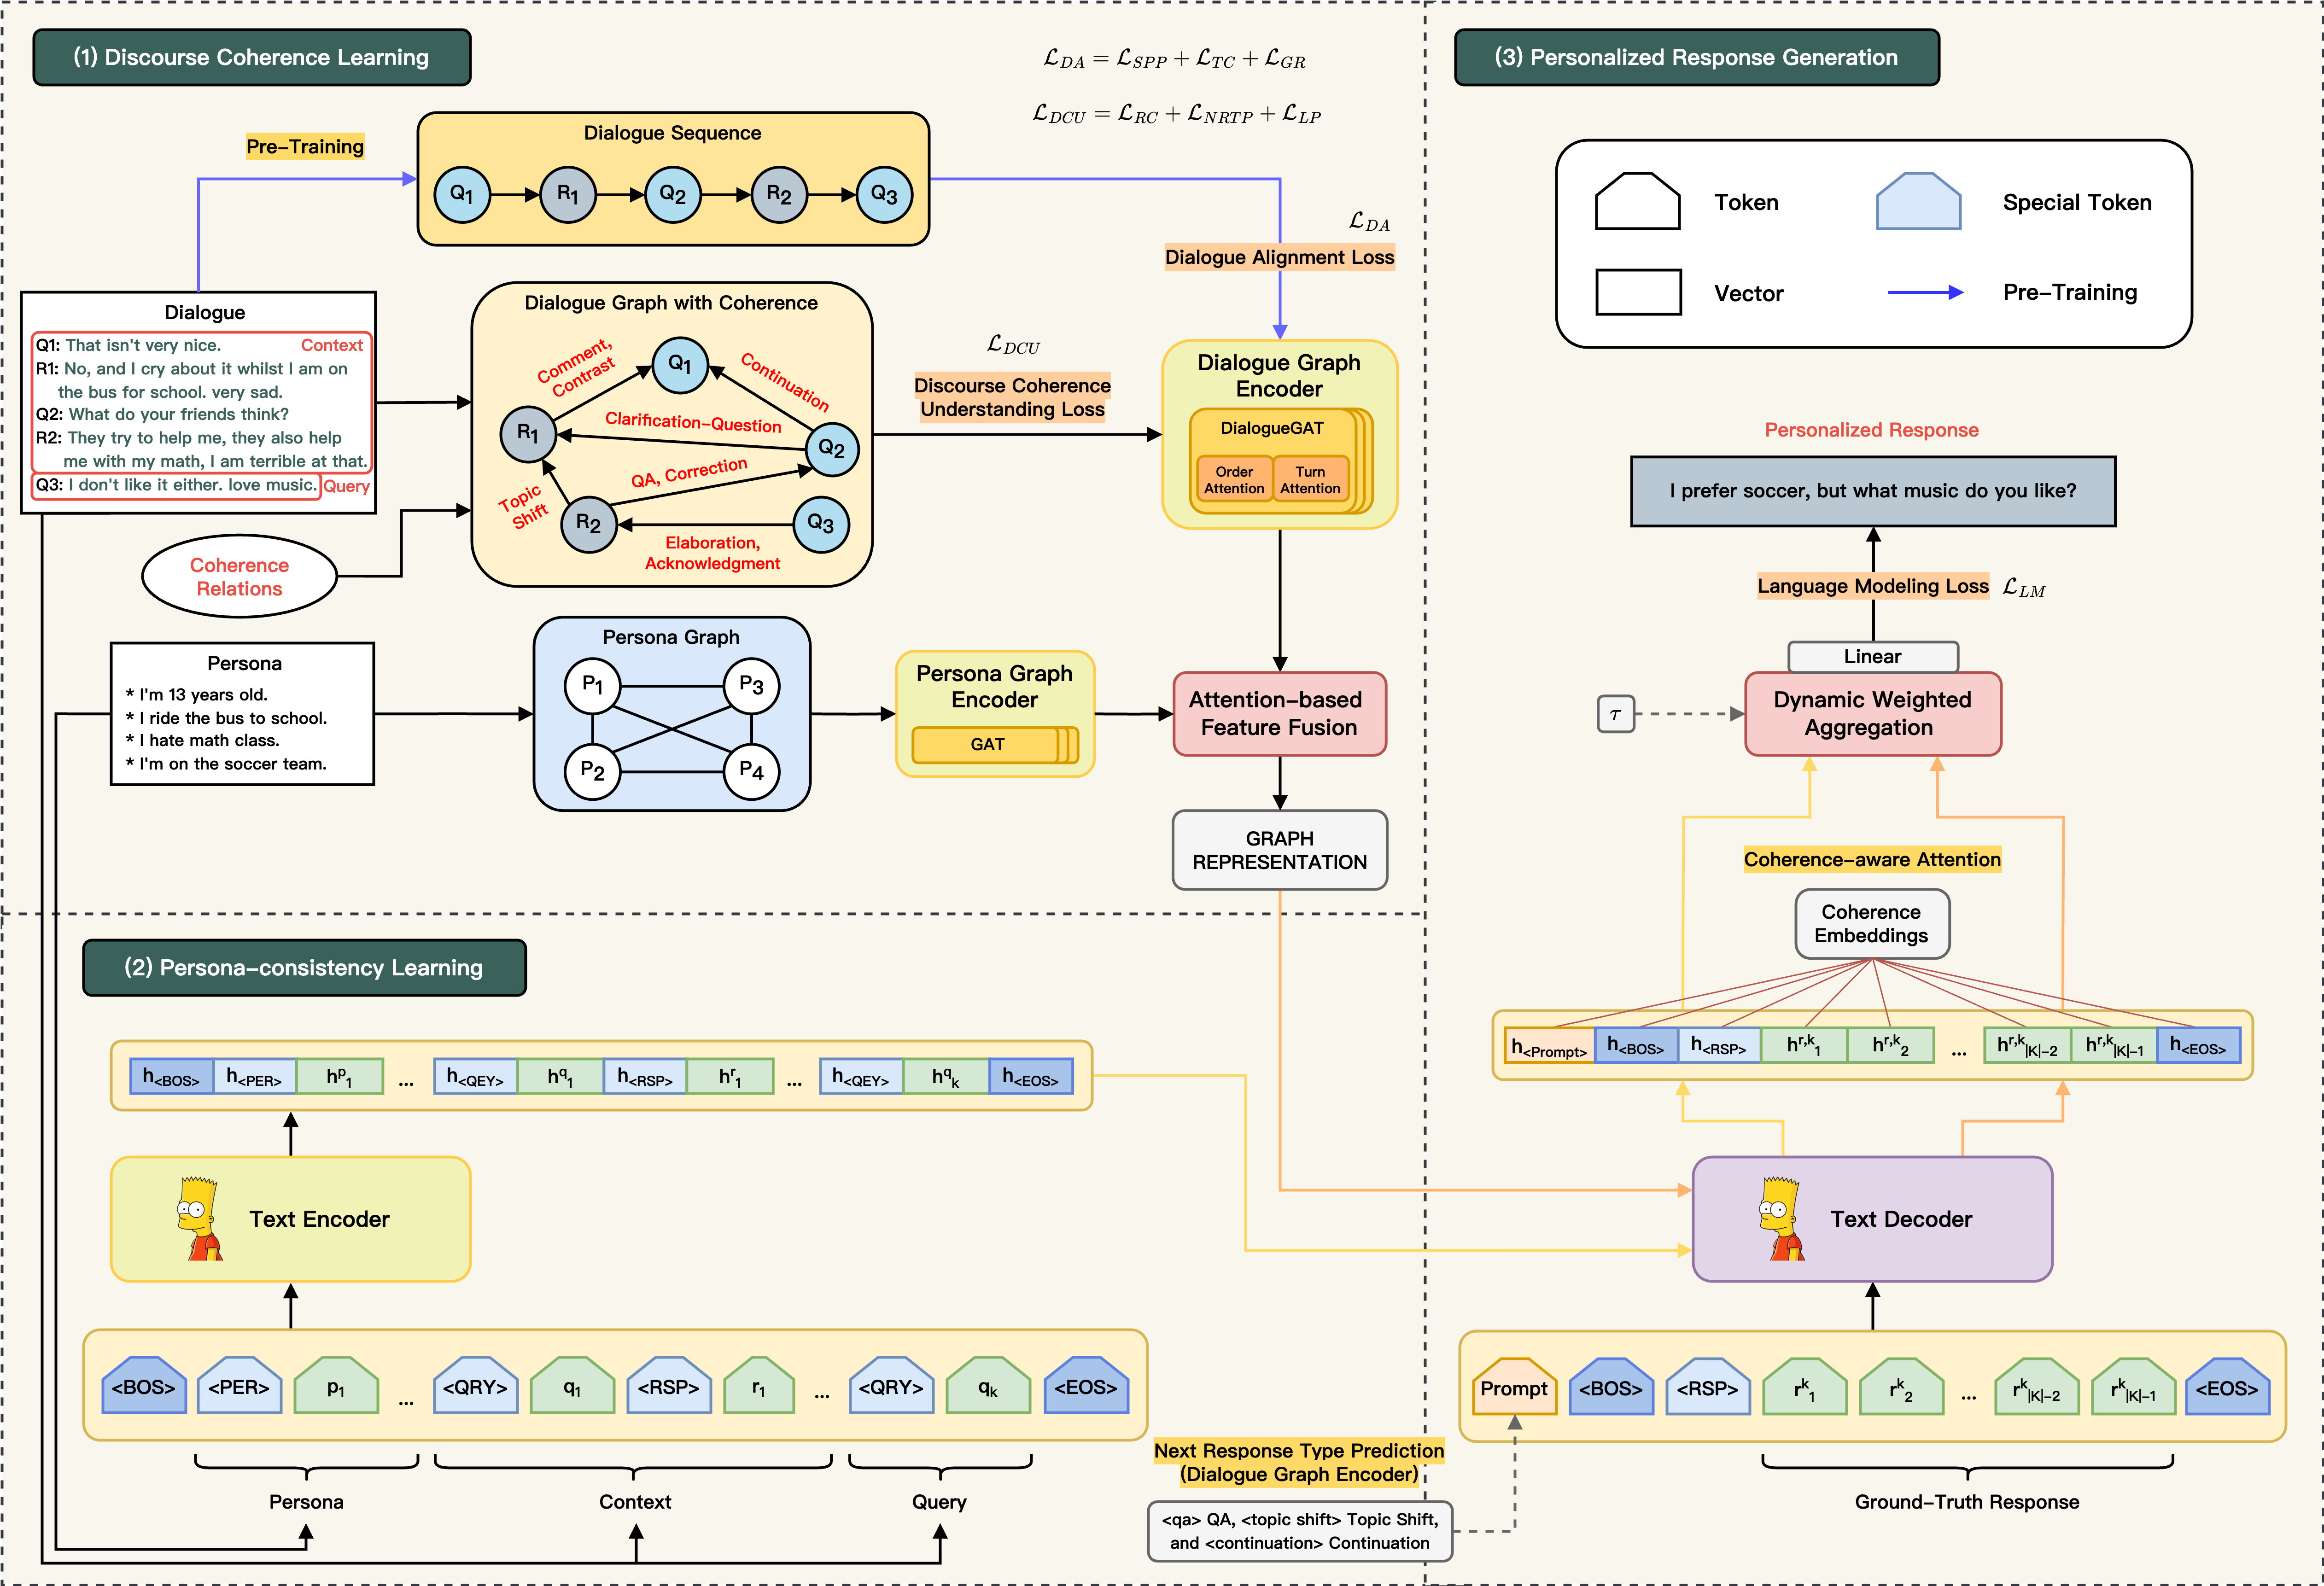
\includegraphics[width=0.54\textwidth]{./images/research_model_arch-v4.png}
    \caption{The overall architecture of our model - MUDI.}
    \label{fig:proposed_model_arch}
\end{figure*}

\section{Methodology}

\subsection{Task Formulation}
The task involves generating a personalized response, denoted as $r_{|K|}$, given the persona descriptions $P = \{p_{1}, p_{2}, ... , p_{|P|}\}$ and a multi-turn dialogue context $C = \{q_{1}, r_{1}, q_{2}, r_{2}, ... , q_{|K|−1}, r_{|K|−1}, q_{|K|}\}$. In this context, $q$ and $r$ represent the user query and the chatbot response, respectively. The core goal of personalized response generation is to accurately estimate the probability distribution $p(r | C, P)$, facilitating the generation of specifically tailored responses that reflect the persona information and dialogue history. 

An ideal personalized response should be not only natural but also consistent with the persona. To generate a more coherent response, we incorporate the discourse relations in dialogue. With specific response types $T = \{t_{1}, t_{2}, ... , t_{|T|}\}$ identified, our goal extends to producing a response $r_{|K|}$ that seamlessly integrates these types across the dialogue. Consequently, we aim to optimize the probability $p(r | C, P, T)$, enhancing both the personalization and coherence of the responses generated.

\subsection{Model Overview}
We propose a framework based on Multiple Discourse Relations Graph Learning, namely \textbf{MUDI}, as illustrated in Fig. \ref{fig:proposed_model_arch}. Initially, we discuss Discourse Coherence Learning, which employs a dialogue-enhanced graph encoder to learn coherence information from the dialogue. Subsequently, we explore Persona Consistency Learning, examining the relationship between persona and context. Finally, we describe our Personalized Response Generation process, which integrates information from the aforementioned steps. This process utilizes a coherence-aware mechanism to guide the generation process and balance the persona and coherence information effectively.

\subsection{Discourse Coherence Learning}
Our method leverages discourse relations to enhance the coherence of dialogue generation. We employ a Graph Neural Network (GNN) model specifically designed to learn these relations. To further improve the GNN's ability to understand dialogue structure, we have enhanced the existing model by incorporating a mechanism to capture dialogue structure. Additionally, we adopt a pretrain-finetune strategy to optimize performance. The detailed description of these enhancements is as follows.


\subsubsection{Coherence Relations Annotation} \label{sec:coherence_reltaions_annotation}
% To facilitate the model's understanding of how two sentences in a conversation are effectively connected, we employ Large Language Models (LLMs) such as GPT-4, Mixtral-8x7b, and LLaMA-3 to assist in annotating coherence relations. There are, in total, 16 discourse relations according to STAC \cite{asher-etal-2016-discourse}, namely, \textbf{comment}, \textbf{clarification-question}, \textbf{elaboration}, \textbf{acknowledgment}, \textbf{continuation}, \textbf{explanation}, \textbf{conditional}, \textbf{question-answer}, \textbf{alternation}, \textbf{question-elaboration}, \textbf{result}, \textbf{background}, \textbf{narration}, \textbf{correction}, \textbf{parallel} and \textbf{contrast}. On top of these relationships, we add \textbf{topic-shift} to represent coherent topic transitions between conversations. Each pair of utterances could be annotated with zero to three different relations. 
To facilitate the model's understanding of how two sentences in a conversation are effectively and coherently connected, we employ Large Language Models (LLMs) such as GPT-4, Mixtral-8x7b, and LLaMA-3 to assist in annotating coherence relations. According to STAC \cite{asher-etal-2016-discourse}, there are 16 discourse relations proposed. To these, we add a \textbf{topic-shift} to represent coherent topic transitions between conversations. Each pair of utterances can be annotated with up to three different relations.

\subsubsection{Dialogue Graph Modeling}
To enable the model to capture discourse coherence information within conversations when generating responses, and inspired by the success of previous graph-based discourse modeling efforts \cite{dong-etal-2021-discourse,feng-etal-2021-dialogue,li-etal-2021-dadgraph}, we employ a Graph encoder to learn the interactive relationships between discourses. To account for sentence-level semantics, we utilize the Sentence-Transformer \cite{reimers-2019-sentence-bert} as an encoder to extract contextualized global semantics from both utterances and personas, thereby initializing the node features.

In our method, we found that the powerful GNN models that have been proposed are not specifically designed for dialogue structure and may not fully capture the intricate structure and complex long-term interactions in conversations. To overcome this, we enhance the GATv2 \cite{brody-etal-2022-gatv2} model by incorporating structures that specifically capture dialogue information. Specifically, we introduce two key modifications to capture the dialogue structure: Order information and Turn information, both integrated via an attention mechanism. We call this dialogue-enhanced GNN is \textbf{DialogueGAT}. The specific introduction to these two mechanisms is as follows:

\subsubsection{Order-Attention}
To model the sequential nature of dialogues, we introduce auxiliary edges connecting each utterance to its $k{\text -}hop$ neighboring utterances based on their order. This indicator could formalized as Eq. \ref{eq:add_order_auxiliary_edges}. Then $d=k+1$, where $d$ represents the difference.

\begin{equation}\label{eq:add_order_auxiliary_edges}
I(i, j, d) = 
\begin{cases} 
1 & \text{if } \operatorname{order}(j) > \operatorname{order}(i) \\
  & \quad \text{and } |\operatorname{order}(i) - \operatorname{order}(j)| < d \\
0 & \text{otherwise}
\end{cases}
\end{equation}

% The attention scores between nodes are calculated based on the exponential decay of the order difference, as described in Eq. \ref{eq:dialoguegat_order_exp_decay}, \ref{eq:dialoguegat_order_act}, \ref{eq:dialoguegat_attn}, and \ref{eq:dialoguegat_hidden_states}. Here, $\lambda$ represents the decay rate.

The attention scores between nodes are calculated based on the exponential decay of the order difference, as described in Eq. \ref{eq:dialoguegat_order_exp_decay} and \ref{eq:dialoguegat_order_act}. Here, $\lambda$ represents the decay rate. Moreover, wZe utilize the standard methods for computing attention scores and updating hidden states. 

\begin{equation}\label{eq:dialoguegat_order_exp_decay}
    s_{ij} = \exp(-\lambda \cdot |\operatorname{order}(i) - \operatorname{order}(j)|) \cdot I(i, j, d)
\end{equation}

\begin{equation}\label{eq:dialoguegat_order_act}
    e(h_i, h_j) = (\alpha^T \cdot \text{LeakyReLU}(W \cdot [h_i \parallel h_j])) \cdot s_{ij}
\end{equation}

\subsubsection{Turn-Attention}
We also incorporate turn information by adding bidirectional auxiliary edges between utterance nodes within the same turn, as described in Eq. \ref{eq:add_turn_auxiliary_edges}

\begin{equation}\label{eq:add_turn_auxiliary_edges}
    t_{ij} = 
    \begin{cases} 
    1 & \text{if } \text{turn}(i) = \text{turn}(j) \\
    0 & \text{otherwise}
    \end{cases}
\end{equation}

Then, we calculate the attention scores between nodes of the same conversational turn in the same manner. These calculations are detailed in Eq. \ref{eq:dialoguegat_turn_act}.

\begin{equation}\label{eq:dialoguegat_turn_act}
    e(h_i, h_j) = (\alpha^T \cdot \text{LeakyReLU}(W \cdot [h_i \parallel h_j])) \cdot t_{ij}
\end{equation}

\subsubsection{Pre-training Phase}
% During the pre-training phase, our objective is to enhance the Graph encoder's ability to comprehend and capture the structure of dialogue data effectively. To achieve this, we perform pre-training on the large-scale dialogue dataset Reddit Conversation Corpus (5-turns) \cite{dziri-etal-2019-augmenting}. Drawing inspiration from the strategies outlined in \cite{wu-etal-2023-gnn-pretrain}, we have designed three specific self-supervised pretraining tasks to aid the model in understanding the intricate dialogue structure. These tasks include Shortest Path Prediction (SPP), which helps the model infer the most direct connections within dialogue sequences; Turn Classification (TC), which assists in recognizing the speaker's changes and continuities; and Graph Reconstruction (GR), aimed at enabling the model to rebuild dialogue sequences from scattered data points. Initially, we convert the raw dialogue data into structured dialogue sequences, and we employ a Graph Encoder to extract hidden states from the dialogue sequence. These hidden states are then utilized in three specific tasks, each with its own loss calculation:

% \begin{itemize}
%     \item \textbf{Shortest Path Prediction}: This task involves predicting the shortest paths between sampled pairs of nodes from multiple dialogue graphs within a batch. Nodes are sampled across different graphs, and the model first concatenates the hidden states of the sampled nodes to form an input vector for the MLP. The predicted shortest path length between a sampled pair of nodes \(i\) and \(j\) is given by Eq. \ref{eq:gnn_pre_concat} \ref{eq:gnn_pre_spp_mlp}.
%     \begin{equation}\label{eq:gnn_pre_spp_mlp}
%         \hat{y}_{ij}^{\text{SPP}} = \text{MLP}(h_{ij})        
%     \end{equation}
%     The loss for this task, denoted as \( \mathcal{L}_{\text{SPP}} \), is computed using the mean squared error (MSE) over the sampled node pairs within the batch:
%     \begin{equation}
%         \mathcal{L}_{\text{SPP}} = \sum_{(i, j) \in S} (y_{ij}^{\text{SPP}} - \hat{y}_{ij}^{\text{SPP}})^2
%     \end{equation}
%     Where \( S \) is the set of sampled node pairs from the batch. If the sampled nodes \(i\) and \(j\) belong to different graphs, the ground truth shortest path length \( y_{ij}^{\text{SPP}} \) is assumed to be 0, reflecting the absence of a path between graphs.

%     \item \textbf{Turn Classification}: This task involves classifying whether two sampled nodes within a batch correspond to utterances that occur in the same turn of a conversation. The model concatenates the hidden states of the sampled nodes to form an input vector for the MLP (Eq. \ref{eq:gnn_pre_concat} \ref{eq:gnn_pre_tc_mlp}), which predicts the probability that the two utterances belong to the same turn:
%     \begin{equation} \label{eq:gnn_pre_tc_mlp}
%         \hat{y}_{ij}^{\text{TC}} = \text{MLP}(h_{ij})
%     \end{equation}
%     The loss for this task, denoted as \( \mathcal{L}_{\text{TC}} \), is calculated using binary cross-entropy:
%     \begin{equation}
%         \mathcal{L}_{\text{TC}} = -\sum_{(i, j) \in S} \left( y_{ij}^{\text{TC}} \log(\hat{y}_{ij}^{\text{TC}}) + (1 - y_{ij}^{\text{TC}}) \log(1 - \hat{y}_{ij}^{\text{TC}}) \right)
%     \end{equation}
%     Where \( S \) is the set of sampled node pairs from the batch, \( y_{ij}^{\text{TC}} \) represents the ground truth label indicating whether the utterances of nodes \( v_i \) and \( v_j \) belong to the same turn, and \( \hat{y}_{ij}^{\text{TC}} \) is the predicted probability. Optimizing this turn classification loss helps to enhance the graph encoder's ability to identify directly related utterances within the dialogue.

%     \item \textbf{Graph Reconstruction}: The objective of this task is to reconstruct the adjacency matrix of the dialogue graph using a method inspired by the Variational Graph Auto-Encoders (VGAE) described in Kipf et al. \cite{kipf-etal-2016-vgae}. We employ an inner product decoder to estimate the adjacency matrix from the hidden representations of the nodes. This approach calculates the probability of an edge existing between any two nodes based on their hidden states. The graph reconstruction loss, \( \mathcal{L}_{\text{GR}} \), is then calculated using binary cross-entropy:
%     \begin{equation}
%         \mathcal{L}_{\text{GR}} = -\sum_{i=1}^N \sum_{j=1}^N \left( A_{ij} \log(\sigma(h_i^T h_j)) + (1 - A_{ij}) \log(1 - \sigma(h_i^T h_j)) \right)
%     \end{equation}
%     This loss function quantifies the error in reconstructing the adjacency matrix, thereby guiding the model toward learning accurate node embeddings that reflect the actual graph structure.

% \end{itemize}

% Consider the pretraining tasks and their respective losses, the total loss $\mathcal{L}_{\text{DA}}$ (Dialogue Alignment) is then given by the sum of these individual losses:
% \begin{equation}
%     \mathcal{L}_{\text{DA}} = \mathcal L_{\text{SPP}} + \mathcal L_{\text{TC}} + \mathcal L_{\text{GR}}
% \end{equation}

During the pre-training phase, our objective is to enhance the Graph encoder's ability to effectively comprehend and capture dialogue structure. To achieve this, we perform pre-training on the large-scale dialogue dataset Reddit Conversation Corpus (5-turns) \cite{dziri-etal-2019-augmenting}. 

\begin{equation}\label{eq:gnn_pre_enc}
    H = \text{GNN}_{\theta}(X^{\text{pre}},A^{\text{pre}})
\end{equation}

% Drawing inspiration from the strategies outlined in \cite{wu-etal-2023-gnn-pretrain}, we have designed three specific self-supervised pretraining tasks to aid the model in understanding the intricate dialogue structure. These tasks include Shortest Path Prediction (SPP), which helps the model infer the most direct connections within dialogue sequences; Turn Classification (TC), which assists in recognizing the speaker's changes and continuities; and Graph Reconstruction (GR), aimed at enabling the model to rebuild dialogue sequences from scattered data points. 
% Initially, we convert the raw dialogue data into structured dialogue sequences, and we employ a Graph Encoder to extract hidden states from the dialogue sequence. Each task employs specific loss calculations to optimize the encoder’s performance in capturing dialogue dynamics:

%     \begin{equation}
%         \mathcal{L}_{\text{SPP}} = \sum_{(i, j) \in S} (y_{ij}^{\text{SPP}} - \hat{y}_{ij}^{\text{SPP}})^2
%     \end{equation}

%     \begin{equation}
%     \begin{aligned}
%         \mathcal{L}_{\text{TC}} &= -\sum_{(i, j) \in S} \left( y_{ij}^{\text{TC}} \log(\hat{y}_{ij}^{\text{TC}}) \\
%         &+ (1 - y_{ij}^{\text{TC}}) \log(1 - \hat{y}_{ij}^{\text{TC}}) \right)
%     \end{aligned}
%     \end{equation}

%     \begin{equation}
%     \begin{aligned}
%         \mathcal{L}_{\text{GR}} &= -\sum_{i=1}^N \sum_{j=1}^N \Bigl( A_{ij} \log(\sigma(h_i^T h_j)) \\
%         &\quad + (1 - A_{ij}) \log(1 - \sigma(h_i^T h_j)) \Bigr)
%     \end{aligned}
%     \end{equation}

Drawing inspiration from the strategies outlined in Wu et al. \cite{wu-etal-2023-gnn-pretrain}, we have designed three specific self-supervised pretraining tasks to aid the model in understanding the intricate dialogue structure. These tasks include:

\begin{itemize}
\item  \textbf{Shortest Path Prediction}: This task enables the model to infer the most direct connections within dialogue sequences, using Mean Squared Error loss to enhance its ability to identify and predict the shortest paths between dialogue nodes. The associated loss is denoted as $\mathcal{L}_{\text{SPP}}$.

\item \textbf{Turn Classification}: This task helps recognize the speaker's changes and continuities within dialogues. It is optimized with Cross-Entropy loss to accurately classify whether successive utterances belong to the same speaker. The loss denoted as $\mathcal{L}_{\text{TC}}$.

\item \textbf{Graph Reconstruction}: This task aimed at enabling the model to rebuild dialogue sequences from scattered data points, this task utilizes Cross-Entropy loss to improve the model's capacity for reconstructing accurate dialogue structures. The loss denoted as $\mathcal{L}_{\text{GR}}$.
\end{itemize}

The total loss for the pre-training tasks, denoted as $\mathcal{L}_{\text{DA}}$ (Dialogue Alignment) is then given by the sum of these individual losses:
\begin{equation}
    \mathcal{L}_{\text{DA}} = \mathcal L_{\text{SPP}} + \mathcal L_{\text{TC}} + \mathcal L_{\text{GR}}
\end{equation}

\subsubsection{Fine-tuning Phase}
% During the finetuning stage, we utilize a personalized dialogue dataset annotated with coherence relations to learn the discourse relations in dialogue. The dataset allows us to finetune the pretrained Graph Encoder $\text{GNN}_{\theta}$ using enhanced data that includes not only the node features $X_{C}^{ft}$ and adjacency matrix $A_{C}^{ft}$ but also coherence relations $R$. Specifically, the node features $X_{C}^{ft}$ and adjacency matrix $A_{C}^{ft}$ are derived from the dialogue context $C$, where each node is connected to its $k{\text -}hop$ nearest neighbors to reflect the local conversational structure. This connectivity pattern helps in capturing the intricate dynamics of dialogue interactions. Due to the significant class imbalance in the labeled coherence relations, where some categories are overrepresented such as "Topic Shift", which may lead to the model excessively focusing on these categories during training, we address this issue by randomly pruning edges that are solely labeled with a high-frequency category. We refer to this graph as the "Dialogue Graph", and its specific visual representation can be seen in the yellow graph on the upper left of Figure \ref{fig:proposed_model_arch}. This approach helps in balancing the distribution of classes and refining the model's understanding of diverse conversational patterns. The finetuning process updates the encoder to $\text{GNN}_{\theta'}$, adapting it more closely to the specificities of the personalized dialogues:
During the fine-tuning stage, we use a personalized dialogue dataset annotated with coherence relations $R$ to refine our pretrained Graph Encoder, $\text{GNN}_{\theta}$. Each node connects to its $k{\text -}hop$ neighbors, reflecting the local conversational structure and aiding in capturing dialogue dynamics. To address class imbalance in coherence relations, such as the overrepresented "Topic Shift," we prune edges labeled exclusively with high-frequency categories to balance class distribution and enhance the model's understanding of diverse conversational patterns. The fine-tuning process updates the encoder to $\text{GNN}_{\theta'}$, better adapting it to personalized dialogues as shown:
\begin{equation}\label{eq:gnn_ft_enc}
    H_{\text{C}} = \text{GNN}_{\theta'}(X_{C}^{\text{ft}}, A_{C}^{\text{ft}}, R)
\end{equation}

In addition, we transform persona sentences from the dialogue into a complete graph, allowing us to leverage a GAT \cite{brody-etal-2022-gatv2}, denoted as $\text{GNN}_{\psi}$. This graph encoder applies its attention mechanism across all connections to better capture the nuances and importance of each persona sentence, enhancing sensitivity to persona-specific information.
\begin{equation}
H_{\text{P}} = \text{GNN}_{\psi}(X_{P}, A_{P})
\end{equation}

% Next, we employ an attention-based feature fusion mechanism to integrate the utterance node representations of a specific speaker in the dialogue graph with the corresponding node representations in the persona graph. By using attention, the model can focus more on persona information that is relevant to this particular utterance. Specifically, we use a cross-attention approach where the persona information serves as the key and value, and the utterance information serves as the query. The feature fusion is then performed using a multi-head attention mechanism to obtain the personalized node representations, denoted as $H_{\text{D}}$:
Next, we employ an attention-based feature fusion mechanism to integrate the utterance node representations of a specific speaker in the dialogue graph with those in the persona graph. This allows the model to focus on persona information relevant to the utterance. The feature fusion is performed using a multi-head attention mechanism to obtain personalized node representations, denoted as $H_{\text{D}}$.
\begin{equation}
\begin{aligned}
    H_{\text{D}} &= \text{MultiHead}(Q,K,V) \\
    \text{where} \quad 
    Q &= H_{\text{C}} \cdot W^Q_i, \quad
    K = H_{\text{P}} \cdot W^K_i, \\
    V &= H_{\text{P}} \cdot W^V_i
\end{aligned}
\end{equation}

Furthermore, we learn coherence through three tasks:

\begin{itemize}
    % \item \textbf{Coherence Relations Classification}: This task is a multi-label classification task. Given two nodes, the graph encoder predicts which of the 17 types of coherence relations exist between them. The loss for this task denoted as \( \mathcal{L}_{\text{RC}} \), is calculated using binary cross-entropy. Optimizing this coherence relations classification loss helps to enhance the graph encoder's ability to identify and distinguish different types of relations within the dialogue context. In our implementation, we encountered a severe label imbalance problem in the coherence relations, exhibiting a long-tail distribution. For example, Topic Shift dominated most labels, leading to model prediction bias towards a few frequent categories. Therefore, we incorporated the Class-balance loss proposed by \cite{cui-etal-2019-cbloss}, which considers the weights between classes to mitigate the issue of the model being dominated by a minority of high-frequency labels. 
    \item \textbf{Coherence Relations Classification}: This task involves multi-label classification where the graph encoder predicts which of the 17 coherence relations exist between two nodes. The task utilizes Cross-Entropy for the loss, denoted as \( \mathcal{L}_{\text{RC}} \), to enhance the encoder’s ability to identify and distinguish relation types within the dialogue. We encountered severe label imbalance in coherence relations, notably with Topic Shift being overly dominant. To address this, we adopted the Class-balance loss from \cite{cui-etal-2019-cbloss}, which adjusts weights between classes to reduce bias toward frequently occurring labels.

    % \item \textbf{Next Response Type Prediction}: This task aims to predict the possible types of the next response. This is also a multi-label classification task, where the model predicts which of the 17 types of coherence relations will be present in the next response. Specifically, we first extract node representations from $H_D$ that have direct sequential relationships in the original dialogue to form a dialogue sequence $S$. Subsequently, we apply two methods to predict the response type: (1) Direct Prediction: The model predicts the kind of the next response based on the current utterance node. (2) Sequential Prediction (auto-regressive style): The model predicts the type of the next response based on all previous utterances. The loss for this task, denoted as $\mathcal{L}{\text{NRTP}}^{\text{direct}}$ and $\mathcal{L}{\text{NRTP}}^{\text{seq}}$, is computed using binary cross-entropy.
    \item \textbf{Next Response Type Prediction}: This task aims to predict the possible types of the next response. We first derive node representations from $H_D$ with direct sequential relationships in the dialogue to form a sequence $S$. The model then uses two approaches for prediction: (1) Direct Prediction, where it determines the next response type based solely on the current utterance node, and (2) Sequential Prediction (auto-regressive style), where it considers all previous utterances. The losses for these methods, denoted as $\mathcal{L}_{\text{NRTP}}^{\text{direct}}$ and $\mathcal{L}_{\text{NRTP}}^{\text{seq}}$, are calculated using Cross-Entropy.

    % \item \textbf{Link Prediction}: This task is similar to the Graph Reconstruction task in the pretraining phase. The objective is to enable the model to capture the discourse structure of the dialogue by predicting the discourse relations between adjacent utterances. The model learns to predict whether an edge exists between two utterance nodes in the dialogue graph, thereby capturing the underlying dialogue structure and the coherence relations between adjacent utterances.
    \item \textbf{Link Prediction}: This task is similar to the Graph Reconstruction task in the pretraining phase, aiming to capture the discourse structure of the dialogue. The model predicts whether an edge exists between two adjacent utterance nodes in the dialogue graph, thereby capturing the underlying structure and coherence relations between the utterances. The prediction method follows the same approach as the Graph Reconstruction task, using an inner product decoder to estimate the existence of an edge based on the representations of two nodes. The link prediction loss, \( \mathcal{L}_{\text{LP}} \), is then calculated using Cross-Entropy.

\end{itemize}

In summary, through the above training process, we enhance the Dialogue Graph Encoder's ability to understand the structure of dialogues and improve its capability to grasp the implicit discourse relations between utterances. Considering the fine-tuning tasks and their respective losses, the total loss $\mathcal{L}_{\text{DCU}}$ (Discourse Coherence Understanding) of this Dialogue Graph Encoder is then given by the weighted sum of these individual losses:
\begin{equation}
    \mathcal{L}_{\text{DCU}} = \alpha \mathcal{L}_{\text{RC}} + \beta \mathcal{L}_{\text{NRTP}}^{\text{direct}} + \gamma \mathcal{L}_{\text{NRTP}}^{\text{seq}} + \delta \mathcal{L}_{\text{LP}}
\end{equation}

where \(\alpha\), \(\beta\), \(\gamma\), and \(\delta\) are the weights for the respective loss components.

\subsection{Persona-consistency Learning}
% In this stage, the objective is to learn the implicit relationships between persona and dialogue. We use BART \cite{lewis-etal-2020-bart} as the backbone model for this stage and for subsequent personalized response generation. Following the approaches used in previous research \cite{chen-etal-2023-memorize}, the input to the BART encoder is the concatenation of the persona descriptions $P$ and dialogue context $C$, which is structured as follows:
% \begin{align*}
%     E_{\text{TextEncoder}} = [e_{\text{[BOS]}}, e_{\text{[PER]}}, e_{\text{p1}}, e_{\text{p2}}, ... , e_{\text{[QRY]}}, e_{\text{q1}}, e_{\text{[RSP]}}, \\ e_{\text{r1}}, ... , e_{\text{[QRY]}}, e_{\text{q}|\text{K}|}, e_{\text{[EOS]}}]
% \end{align*}
% where [PER], [QRY], and [RSP] are three special tokens that indicate the beginning of persona, query, and response, respectively.
In this stage, the objective is to learn the implicit relationships between persona and dialogue. We use BART \cite{lewis-etal-2020-bart} as the backbone model for this stage and for subsequent personalized response generation. Following the approaches used in previous research \cite{chen-etal-2023-memorize}, the input to the Text encoder is the concatenation of the persona descriptions $P$ and dialogue context $C$, which is structured as follows: $E_{\text{TextEncoder}} = [e_{\text{[BOS]}}, e_{\text{[PER]}}, e_{\text{p1}}, e_{\text{p2}}, ... , e_{\text{[QRY]}}, e_{\text{q1}}, e_{\text{[RSP]}}, e_{\text{r1}}, ... , e_{\text{[QRY]}}, \\e_{\text{q}|\text{K}|}, e_{\text{[EOS]}}]$. where [PER], [QRY], and [RSP] are three special tokens that indicate the beginning of persona, query, and response, respectively.


\subsection{Personalized Response Generation}
% After the aforementioned dialogue representation learning processes, we obtain the coherence-aware dialogue representation through the Dialogue Graph Encoder and the persona-aware dialogue representation through the Text Encoder (BART Encoder). In this stage, our objective is to generate personalized responses guided by the learned implicit representations from the previous steps. First, we refer to the prompt-based conditional dialogue generation approach. We design a prompt to provide guiding signals for the response generation process. Building on the Dialogue Graph Encoder's next response type predictions, the Prompt Tuning module generates a comprehensive description. This description not only instructs the response generator on how to approach the given task but also guides its generation process by specifying the response types and leveraging both the dialogue context and the persona information.
After completing the dialogue representation learning processes, we obtain coherence-aware dialogue representations through the Dialogue Graph Encoder and persona-aware representations through the Text Encoder. Our objective is to generate personalized responses informed by these implicit representations. Initially, we employ a prompt-based conditional dialogue generation approach, designing a prompt that provides guiding signals for the response generation process. Building on the predictions from the Dialogue Graph Encoder about the next response type, our Prompt Tuning module generates a comprehensive description. This description instructs the response generator on task approach and guides the generation process by specifying response types, leveraging both dialogue context and persona information. Therefore, the input sequence for the personalized response generator (Text Decoder) is structured as follows: $E_{\text{Generator}} = [e_{\text{[PROMPT]}}, e_{\text{[BOS]}}, e_{\text{[RSP]}}, e_{\text{1}}^{\text{k}}, e_{\text{2}}^{\text{k}}, ... , e_{|\text{K}|-1}^{\text{k}}, e_{|\text{K}|}^{\text{k}}, e_{\text{[EOS]}}]$.

% Therefore, the input sequence for the personalized response generator (BART Decoder) is structured as follows:
% \begin{align*}
%     E_{\text{Generator}} = [e_{\text{[PROMPT]}}, e_{\text{[BOS]}}, e_{\text{[RSP]}}, e_{\text{1}}^{\text{k}}, e_{\text{2}}^{\text{k}}, ... ,\\ e_{|\text{K}|-1}^{\text{k}}, e_{|\text{K}|}^{\text{k}}, e_{\text{[EOS]}}]
% \end{align*}

% In an encoder-decoder transformer architecture like BART, the decoder references information from the encoder through cross-attention when predicting the next token. To ensure that the generator considers more coherence information while predicting the next token, we apply cross-attention to the dialogue representations generated by the previous two encoders at each transformer block. Thus, during the response generation process, each layer of the decoder performs cross-attention not only on the standard encoder outputs but also on the coherence-aware dialogue representation from the Dialogue Graph Encoder.

% Additionally, we propose the Coherence-aware Attention mechanism. We first use learnable embeddings to capture the semantic information of coherence relations. Special tokens representing coherence relations are incorporated into the aforementioned prompt, combining the token embeddings of these special tokens with the coherence embeddings. This mechanism allows the generator to consider the type of response being predicted, such as selecting words that align with an Acknowledgment response type. This dual cross-attention mechanism enables the decoder to leverage comprehensive context and persona information, thereby enhancing the coherence and personalization of the generated responses.
To enhance coherence in the next token prediction, we apply cross-attention to dialogue representations from the Dialogue Graph Encoder at each transformer block. Consequently, each layer of the decoder performs cross-attention on both the standard encoder outputs and the coherence-aware dialogue representation. Furthermore, we introduce a Coherence-aware Attention mechanism that employs learnable embeddings to capture the semantic nuances of coherence relations. Special tokens representing these relations are integrated into the prompt, combining their embeddings with those of coherence relations. This approach enables the generator to consider the type of response being predicted, such as words aligning with an Acknowledgment response type. This dual cross-attention mechanism allows the decoder to leverage both context and persona information more effectively, enhancing the coherence and personalization of generated responses. Finally, inspired by \cite{huang-etal-2023-paa}, we enhance the generator's ability to incorporate both persona-aware and coherence-aware context information during generation through a Dynamic Weighted Aggregation mechanism. Specifically, we aim to address the trade-off between coherence and persona consistency by balancing the information from the Graph Encoder and Text Encoder. We use a threshold hyperparameter $\tau$ and a learnable mask to control the proportion of persona-aware and coherence-aware information considered.

% Finally, to enable the generator to better consider both persona-aware and coherence-aware context information during generation, we are inspired by \cite{huang-etal-2023-paa}. We fuse the decoder hidden states that consider the text encoder information with those that consider the dialogue graph encoder through a Dynamic Weighted Aggregation mechanism. Specifically, we compute a weight $w_{\text{TextEnc}}$ using a sigmoid function over the concatenated hidden states from both encoders (Eq. \ref{eq:dynamic_weighted_aggregation_weight}). Using this weight, we create masked versions of the encoder outputs based on a threshold hyperparameter $\tau$ to control the proportion of persona-aware and coherence-aware information to be considered (Eq. \ref{eq:dynamic_weighted_aggregation_weighting} and \ref{eq:dynamic_weighted_aggregation_mask}). The final output of the generator $O_{\text{Generator}}$ is obtained by adding a residual connection of the original encoder hidden states to the aggregated hidden states, enhancing the coherence and personalization of the generated responses. The detailed formulas are provided in the following equations:

% \begin{equation} \label{eq:dynamic_weighted_aggregation_weight}
%     w_{\text{TextEnc}} = \sigma(\text{MLP}([H_{\text{TextEnc}} \parallel H_{\text{GraphEnc}}]))
% \end{equation}

% \begin{equation} \label{eq:dynamic_weighted_aggregation_weighting}
%     \begin{aligned}
%         O_{\text{TextEnc}} &= w_{\text{TextEnc}} \cdot H_{\text{TextEnc}}, \\
%         O_{\text{GraphEnc}} &= (1 - w_{\text{TextEnc}}) \cdot H_{\text{GraphEnc}}
%     \end{aligned}
% \end{equation}

% \begin{equation} \label{eq:dynamic_weighted_aggregation_mask}
%     \begin{aligned}
%         m_{\text{TextEnc}} &= \mathbb{M}(w_{TextEnc} > \tau), \\
%         m_{\text{GraphEnc}} &= \mathbb{M}(1 - w_{TextEnc} > \tau)
%     \end{aligned}
% \end{equation}

% \begin{equation}
%     \begin{aligned}
%         \hat{O}_{\text{TextEnc}} &= m_{\text{TextEnc}} \odot O_{\text{TextEnc}}, \\
%         \hat{O}_{\text{GraphEnc}} &= m_{\text{GraphEnc}} \odot O_{\text{GraphEnc}}, \\
%         H_{\text{Enc}} &= \hat{O}_{\text{TextEnc}} + \hat{O}_{\text{GraphEnc}}
%     \end{aligned}
% \end{equation}

% \begin{equation} \label{eq:dynamic_weighted_aggregation_output}
%     \begin{aligned}
%         H_{\text{residual}} &= H_{\text{TextEnc}} + H_{\text{GraphEnc}}, \\
%         O_{\text{Generator}} &= H_{\text{Enc}} + H_{\text{residual}}
%     \end{aligned}
% \end{equation}

For personalized response generation, we use a language modeling task to compute the probability distribution over the vocabulary for generating the next word given the current context. This approach encourages the model to generate responses that are contextually relevant. By minimizing this loss function, the model learns to produce responses that are fluent, personalized, coherent with the dialogue history, and consistent with the persona. The loss function can be formally defined as:

\begin{equation}
    \mathcal{L}_{\text{LM}} = - \sum_{t=1}^{T} \log P(y_t | y_{<t}, O_{\text{Generator}})
\end{equation}

\section{Experiments}

\begin{table*}[ht]
\centering
\def\arraystretch{1.3}%
\begin{tabular}{|c|c|c|c|c|c|c|}
\hline
\multicolumn{2}{|c|}{\multirow{2}{*}{\textbf{Model}}}  & \multicolumn{3}{|c|}{\textbf{Text Similarity}} & \multicolumn{1}{c|}{\textbf{Personalization}} & \multicolumn{1}{c|}{\textbf{Coherence}} \\
\cline{3-7}

\multicolumn{2}{|c|}{} & BLEU-1 $\uparrow$ & ROUGE-1 $\uparrow$ & BERTScore $\uparrow$ & C.Score $\uparrow$ & QuantiDCE $\uparrow$ \\
\hhline{|=======|}

\rowcolor[RGB]{242,164,100}
\multicolumn{7}{|c|}{\textbf{Large Language Model (Prompting)}} \\
\hhline{|=======|}

\multicolumn{2}{|c|}{\textbf{GPT-4}} &7.47 &13.52 &84.05 &2.86 &3.41 / 2.92 \\ 
\hhline{|=======|}

\rowcolor{yellow}
\multicolumn{7}{|c|}{\textbf{General Dialogue Generation}} \\
\hhline{|=======|}

\multicolumn{2}{|c|}{\textbf{DialoGPT}} &7.34 &9.46 &83.31 &4.53 &\textbf{\textcolor{red}{3.23}} / 2.79 \\ 
\hline

\multirow{2}{*}{\textbf{PLATO}} & w/ persona &4.35 &4.88 &82.77 &0.56 &1.68 / 1.57 \\ 
\cline{2-7}

\multirow{2}{*}{\textbf{}} & w/o persona  &6.82 &4.99 &81.44 &0.18 &1.87 / 1.77 \\ 
\hhline{|=======|}

\rowcolor[RGB]{204,217,245}
\multicolumn{7}{|c|}{\textbf{Persona-based Dialogue Generation}} \\
\hhline{|=======|}

\multicolumn{2}{|c|}{\textbf{BoB}} &15.30 &13.21 &83.77 &0.51 &2.99 /2.76 \\ 
\hline

\multicolumn{2}{|c|}{\textbf{LMEDR}}		&15.47	&13.28	&85.00 &7.83 &2.89 / 2.90 \\ 
\hline

\multicolumn{2}{|c|}{\textbf{PAA}}          &\underline{16.55}      &13.53   &84.42 &\textbf{\textcolor{red}{15.19}} &2.70 / \underline{2.93}   \\
\hline

\multirow{3}{*}{\textbf{\begin{tabular}{@{}c@{}}MUDI \\ (ours)\end{tabular}}} &SP\textsubscript{$\tau=0.2$}	&15.14	&14.87	&85.07 &\underline{11.87} &3.05 / 2.84	\\
\cline{2-7}

\multirow{3}{*}{} &Emb\textsubscript{$\tau=0.2$}   &\underline{16.55}  &\textbf{\textcolor{red}{17.10}}	&\underline{85.42} &9.70 &\textbf{\textcolor{red}{3.23}} / \textbf{\textcolor{red}{2.94}}	\\
\cline{2-7}

\multirow{3}{*}{} &SP+Emb\textsubscript{$\tau=0.2$}   &\textbf{\textcolor{red}{18.19}}	&\underline{16.59}	&\textbf{\textcolor{red}{85.53}} &9.75 &\underline{3.21} / 2.92 \\
\hline
\end{tabular}
\caption{Automatic evaluation results on ConvAI2 dataset over our implemented approach. The best results in each column are in bold, while the second is underlined.}
\label{table:main-results}
\end{table*}

\subsection{Experimental Setup}
\subsubsection{Dataset}
We perform experiments on the ConvAI2 dataset. ConvAI2 \cite{dinan-etal-2019-convai2} is a chit-chat dataset based on PersonaChat \cite{zhang-etal-2018-personalizing}. The dataset comprises 17,878 and 1,000 multi-turn dialogues for the training and development sets, respectively, with a total of 131,438 and 7,801 utterances. It features 1,155 and 100 unique persona descriptions for the training and development sets, respectively. Each conversation participant who are assigned at least five persona descriptions, which are selected from these unique personas.

\subsubsection{Baselines}
For comparison, we have selected the following baselines: (1) \textbf{Personalized Dialogue Generation methods}: We compare our approach with established text-description-based personalized models such as BOB \cite{song-etal-2021-bob}, LMEDR \cite{chen-etal-2023-memorize}, and PAA \cite{huang-etal-2023-paa}, which are recognized for their strong performance. (2) \textbf{General Dialogue Generation methods}: To ensure a fair evaluation, we include PLATO \cite{bao-etal-2020-plato} and DialoGPT \cite{zhang-etal-2019-dialogpt}. For PLATO, following the original publication's methodology, we prepend the persona descriptions as part of the knowledge to the entire context during inference. For DialoGPT, we adopt a post-processing approach as suggested by \cite{zhou-etal-2023-simoap}. We first generate multiple responses as candidates from DialoGPT for the same context and then select the response that is most consistent with the persona and most relevant to the context as the final output. (3) \textbf{Large Language Models (LLMs)}: We also test the ability of LLMs, specifically GPT-4, in personalized response generation, which utilizes prompting technologies.

\subsubsection{Implementation Details}
% The \textbf{MUDI} is mainly implemented in PyTorch. Our backbone Generator is BART-large\footnote[2]{https://huggingface.co/facebook/bart-large}. For Generator training, we train it using a batch size of 4 on 1 NVIDIA A100 80GB GPU via the AdamW optimizer with a learning rate of \(5 \times 10^{-6}\) and a weight decay of 0.01. For the Dialogue Graph Encoder training, it is conducted on a single NVIDIA RTX 4090 GPU using a batch size of 512. The training also employs the AdamW optimizer, but with a learning rate of \(2 \times 10^{-5}\) and the same weight decay of 0.01. In the Dialogue Graph Encoder, we initially employ the SBERT model "all-mpnet-base-v2"\footnote[3]{https://huggingface.co/sentence-transformers/all-mpnet-base-v2} to encode both the utterances and persona sentences, thereby initializing the node embeddings. We construct the Dialogue Graph by keeping the 3-hop neighbors. The model employs a 2-layer GNN with 4 multi-heads and a hidden dimension of 512. The weights for the different tasks are as follows: the weight of the Coherence Relation Classification task is 1.5, the weight of both types of Next Response Type Prediction tasks is 1.5, and the weight of the Link Prediction task is 1.2. For training the generator, we retain the most recent 5 turns of dialogue as historical context and choose the top-3 predicted response types for the prompt. We set \(\tau = 0.2\) for the Dynamic Weighted Aggregation. 
The \textbf{MUDI}'s backbone Generator is BART-large\footnote[1]{https://huggingface.co/facebook/bart-large}. For Generator training, we train it on 1 NVIDIA A100 80GB GPU. For the Dialogue Graph Encoder training, it is conducted on a single NVIDIA RTX 4090 GPU. In the Dialogue Graph Encoder, we initially employ the SBERT model\footnote[2]{https://huggingface.co/sentence-transformers/all-mpnet-base-v2} to encode both the utterances and persona sentences, thereby initializing the node embeddings. We construct the Dialogue Graph by keeping the 3-hop neighbors. The model employs a 2-layer GNN. For training the generator, we retain the most recent 5 turns of dialogue as historical context and choose the top-3 predicted response types for the prompt. We set \(\tau = 0.2\) for the Dynamic Weighted Aggregation. Other detailed configurations of each method are given in Appendix\footnote[3]{The detailed appendix will be available online.}.

\subsubsection{Automatic Evaluation}
% We assess the quality of dialogue responses from four perspectives: (1) \textbf{Text-similarity}: To evaluate the similarity between the generated responses and the ground-truth responses, we employ BLEU \cite{papineni-etal-2002-bleu} and ROUGE \cite{lin-2004-rouge} metrics, which focus on the word overlap level. Additionally, we utilize BERTScore \cite{zhang-etal-2020-bert-score}, which measures the semantic similarity between generated responses and ground-truth using contextual embeddings from BERT. This helps capture nuances that traditional overlap-based metrics might miss. (2) \textbf{Diversity}: We assess the diversity and informativeness of the generated responses at token, sentence, and corpus levels. We utilize Distinct-n (Dist-$n$) metrics \cite{li-etal-2016-diversity} to measure the proportion of unique n-grams (n=1) relative to the total number of n-grams in the generated responses. Additionally, we employ Entropy-n (Ent-$n$) \cite{zhang-etal-2018-generating} to evaluate the uncertainty or randomness of the distribution of n-grams (n=1) in the generated text. We also calculate the Unique Sentence Ratio (USR) \cite{li-etal-2020-generate}, which quantifies text diversity by measuring the proportion of unique sentences among all predicted responses. (3) \textbf{Coherence}: Previous studies often omit explicit evaluations of Coherence, assuming that Fluency can also measure the coherence of dialogues. However, this approach does not directly account for the coherence of generated responses with the context and query, an aspect often presumed to be covered by fluency. To measure this unexplored dimension, our research incorporates specific coherence metrics to provide a more accurate and holistic assessment of response quality. Specifically, We employ QuantiDCE \cite{ye-etal-2021-towards-quantifiable} which are state-of-the-art metrics in dialogue coherence evaluation. These metrics assess both how logically the responses align with the preceding query or the entire context within the dialogue, and how well the utterances in a conversation are unified, leading to a consistent and coherent interaction. (4) \textbf{Personalization}: To assess the personalization of the generated responses, we apply Consistency Score (C.Score) \cite{madotto-etal-2019-personalizing}, which leverages a NLI model to predict consistency between response and persona.
We assess the quality of dialogue responses from four perspectives: (1) \textbf{Text-similarity}: We using BLEU \cite{papineni-etal-2002-bleu}, ROUGE \cite{lin-2004-rouge}, and BERTScore \cite{zhang-etal-2020-bert-score} to evaluate lexical overlap and semantic similarity between generated and ground-truth responses. (2) \textbf{Diversity}: Measured using Distinct-n (Dist-$n$) \cite{li-etal-2016-diversity} metrics for unique n-grams, Entropy-n (Ent-$n$) \cite{zhang-etal-2018-generating} to assess n-gram distribution, and Unique Sentence Ratio (USR) \cite{li-etal-2020-generate} to evaluate sentence uniqueness. (3) \textbf{Coherence}: We use QuantiDCE metrics \cite{ye-etal-2021-towards-quantifiable} to assess dialogue coherence, focusing on how responses align with preceding queries and the overall context, and the unity of utterances within the conversation. This approach addresses the limitations of traditional fluency-based evaluations. (4) \textbf{Personalization}: We use Consistency Score (C.Score) \cite{madotto-etal-2019-personalizing} to evaluate how well responses align with the persona based on predictions from an NLI model.

% \begin{table}[ht]
% \centering
% \def\arraystretch{1.3}%
% \begin{tabular}{|c|c|c|c|c|}
% \hline
% \multicolumn{2}{|c|}{\multirow{2}{*}{\textbf{Model}}}  &\multicolumn{3}{c|}{\textbf{Diversity}}\\
% \cline{3-5}

% \multicolumn{2}{|c|}{} &Ent-1 $\uparrow$ &Dist-1 $\uparrow$ &USR $\uparrow$ \\
% \hhline{|=====|}

% \rowcolor[RGB]{242,164,100}
% \multicolumn{5}{|c|}{\textbf{Large Language Model (Prompting)}} \\
% \hhline{|=====|}

% \multicolumn{2}{|c|}{\textbf{GPT-4}} &9.40 &16.09 &1.00 \\ 
% \hhline{|=====|}

% \rowcolor{yellow}
% \multicolumn{5}{|c|}{\textbf{General Dialogue Generation}} \\
% \hhline{|=====|}

% \multicolumn{2}{|c|}{\textbf{DialoGPT}} &\textbf{\textcolor{red}{9.05}} &36.84 &\underline{0.99} \\ 
% \hline

% \multirow{2}{*}{\textbf{PLATO}} & w/ persona &4.67 &\textbf{\textcolor{red}{58.18}} &0.61 \\ 
% \cline{2-5}

% \multirow{2}{*}{\textbf{}} & w/o persona &6.73 &43.34 &0.85 \\ 
% \hhline{|=====|}

% \rowcolor[RGB]{204,217,245}
% \multicolumn{5}{|c|}{\textbf{Persona-based Dialogue Generation}} \\
% \hhline{|=====|}


% \multicolumn{2}{|c|}{\textbf{BoB}} &7.89 &41.75 &\underline{0.99} \\ 
% \hline

% \multicolumn{2}{|c|}{\textbf{LMEDR}}  &7.14	&43.08	&0.94\\ 
% \hline

% \multicolumn{2}{|c|}{\textbf{PAA}}    &6.66	&40.27  &0.87 \\
% \hline

% \multirow{3}{*}{\textbf{\begin{tabular}{@{}c@{}}MUDI \\ (ours)\end{tabular}}} &SP\textsubscript{$\tau=0.2$}	&\underline{8.13}		&46.76	&\textbf{\textcolor{red}{1.00}}\\
% \cline{2-5}

% \multirow{3}{*}{} &Emb\textsubscript{$\tau=0.2$}   &7.65	&\underline{51.03}	&\textbf{\textcolor{red}{1.00}}\\
% \cline{2-5}

% \multirow{3}{*}{} &SP+Emb\textsubscript{$\tau=0.2$} 	&7.66	&47.68  &\textbf{\textcolor{red}{1.00}}\\
% \hline
% \end{tabular}
% \caption{Automatic evaluation results for diversity tested on ConvAI2 dataset over our implemented approach. The best results in each column are in bold, while the second is underlined.}
% \label{table:text-diversity}
% \end{table}

\begin{table}[ht]
\centering
\def\arraystretch{1.3}%
\begin{tabular}{|c|c|c|c|c|}
\hline
\multicolumn{2}{|c|}{\multirow{2}{*}{\textbf{Model}}}  &\multicolumn{3}{c|}{\textbf{Diversity}}\\
\cline{3-5}

\multicolumn{2}{|c|}{} &Ent-1 $\uparrow$ &Dist-1 $\uparrow$ &USR $\uparrow$ \\
\hhline{|=====|}

\rowcolor[RGB]{204,217,245}
\multicolumn{5}{|c|}{\textbf{Persona-based Dialogue Generation}} \\
\hhline{|=====|}

\multicolumn{2}{|c|}{\textbf{BoB}} &\underline{7.89} &41.75 &\underline{0.99} \\ 
\hline

\multicolumn{2}{|c|}{\textbf{LMEDR}}  &7.14	&43.08	&0.94\\ 
\hline

\multicolumn{2}{|c|}{\textbf{PAA}}    &6.66	&40.27  &0.87 \\
\hline

\multirow{3}{*}{\textbf{\begin{tabular}{@{}c@{}}MUDI \\ (ours)\end{tabular}}} &SP\textsubscript{$\tau=0.2$}	&\textbf{\textcolor{red}{8.13}}		&46.76	&\textbf{\textcolor{red}{1.00}}\\
\cline{2-5}

\multirow{3}{*}{} &Emb\textsubscript{$\tau=0.2$}   &7.65	&\textbf{\textcolor{red}{51.03}}	&\textbf{\textcolor{red}{1.00}}\\
\cline{2-5}

\multirow{3}{*}{} &SP+Emb\textsubscript{$\tau=0.2$} 	&7.66	&\underline{47.68}  &\textbf{\textcolor{red}{1.00}}\\
\hline
\end{tabular}
\caption{Automatic evaluation results for diversity on the ConvAI2 dataset. Best results are bolded and second-best are underlined.}
\label{table:text-diversity}
\end{table}

\subsection{Main Results}
% Apart from DialoGPT, we use the context of the most recent 5 turns as dialogue history. After testing, we found that DialoGPT starts to talk nonsense when given more than 2 turns of context. Therefore, for DialoGPT, we only use the most recent 2 turns.

In Table \label{table:main-results} we report experimental results on Text Similarity, Personalization, and Coherence evaluation. Our method offers better BLEU, ROUGE, and BERTScore compared with baseline methods. Specifically, MUDI's BLEU-1 and ROUGE-1 scores reach 18.19 and 17.10, respectively, outperforming existing methods by 1.64 and 3.57. As shown in Table \ref{table:text-diversity}, we report the Diversity evaluation. MUDI's USR is 1.0, indicating that it can generate completely unique responses under different queries and personas. Furthermore, our approach achieves the highest scores among all Persona-based dialogue generation methods and significantly surpasses other baselines in Dist-1, outperforming them by 7.95. This performance establishes our method could generate varied and engaging responses. In addition, the results of the Coherence evaluation. Compared to other persona-based methods, MUDI has made significant progress in QuantiDCE, particularly in assessing the coherence between the query and response (left-side scores). This indicates that our approach indeed enables the model to generate responses with enhanced local coherence. Furthermore, MUDI also achieves excellent results in global coherence, which evaluates the coherence between the entire dialogue context and the response (right-side scores). Finally, the results of evaluating Personalization and Feature Coverage. PAA significantly outperforms other methods in scores for Personalization. Upon further examination, we discovered that this is because PAA frequently generates sentences that are exact restatements of the persona description, often ignoring the relevance to the query. As a result, its high scores in Personalization can be attributed to this tendency. Excluding the special case of PAA, MUDI achieves excellent results in Personalization compared to other methods. Combined with the previously discussed results from the Coherence evaluation, this demonstrates that our approach successfully balances discourse relations and persona. It generates responses that effectively consider both aspects simultaneously. Furthermore, our model achieves comparable scores in the Coherence evaluation compared to DialoGPT, which focuses on general dialogue generation.

In summary, compared to existing methods, our approach MUDI not only significantly improves performance in Text Similarity scores but also excels at integrating discourse relations and persona information. This enables us to generate personalized responses that are not only rich in content and diverse but also encompass these aspects. Moreover, in Coherence evaluations, our method achieves scores comparable to those of state-of-the-art models specialized in open-domain dialogue generation.

\begin{figure}[ht]
    \centering
    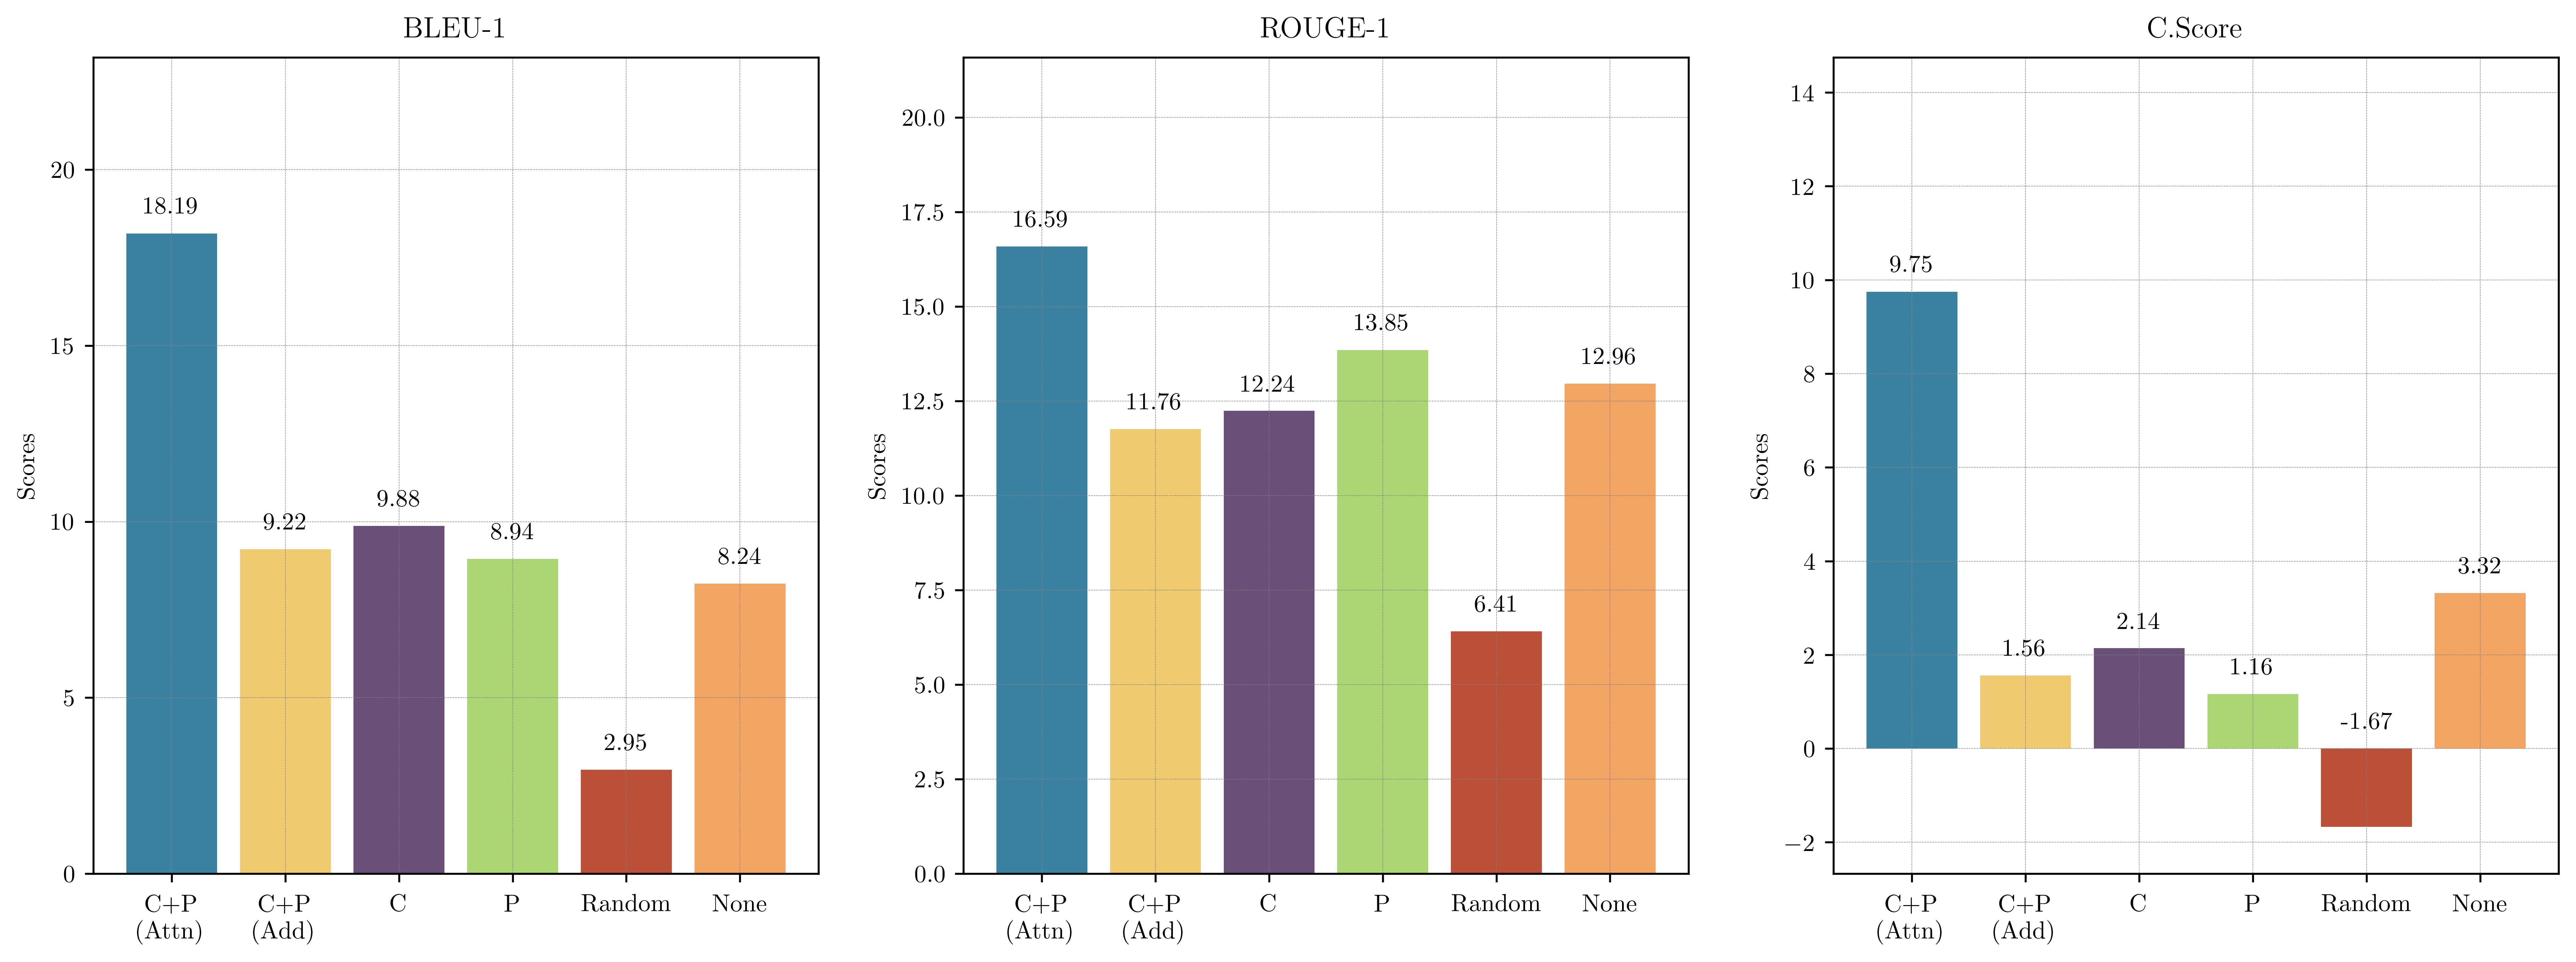
\includegraphics[width=0.48\textwidth]{./images/effectiveness_of_dialogue_graph_encoder.png}
    \caption{Performance analysis of Dialogue Graph Encoder across different settings. Here, "C" represents Context, and "P" represents Persona.}
    \label{fig:effectiveness_of_dialogue_graph_encoder}
\end{figure}

\subsection{Analysis}
\subsubsection{The Effect of Dialogue Graph Encoder}
% We analyze the effectiveness of the Dialogue Graph Encoder (discussed in Section 3.2.2 fine-tuning phase) under various settings. (1) \textbf{Context+Persona (Attention)}: This is our primary method where we utilize an Attention-based Feature Fusion approach to integrate representations from both the Dialogue Graph and the Persona Graph. (2) \textbf{Context+Persona (Add)}: We replace the Attention-based Feature Fusion approach with a simple addition of the persona and context representations. (3) \textbf{Context}: In this setting, we solely rely on the representation from the Dialogue Graph. (4) \textbf{Persona}: Here, we use only the representation from the Persona Graph. (5) \textbf{Random}: A random vector replaces the output of the Dialogue Graph Encoder. (6) \textbf{None}: The Dialogue Graph Encoder is completely removed from the process, allowing the generator to receive only the context and persona information from the Text Encoder. The comprehensive experimental results can be found in Figure \ref{fig:effectiveness_of_dialogue_graph_encoder}. We report the metrics for BLEU-1, ROUGE-1, and Consistency Score (C.Score).

% Our experimental results demonstrate that the attention-based feature fusion approach (Context+Persona (Attention)) significantly outperforms other methods in terms of BLEU-1 and ROUGE-1 scores. These findings confirm that effectively integrating contextual and persona information through an attention mechanism enhances the similarity of the generated responses to the ground-truth responses. In contrast, simpler methods such as addition (Context+Persona (Add)) or those relying solely on context or persona information exhibit lower performance. The scores drastically decrease when random vectors are employed or when the dialogue graph encoder is omitted entirely, which emphasizes the crucial role of structured and meaningful input in producing coherent responses. The consistency scores further elucidate the models' ability to generate responses that align with persona traits. The superior performance of the attention-based method suggests its effectiveness in maintaining persona consistency within the responses. Notably, employing random vectors results in negative C.Score values, indicating that some generated responses are not only irrelevant but also contradictory to the defined personas.

% These outcomes reinforce the importance of utilizing attention-based feature fusion in dialogue systems, especially in tasks that require a nuanced understanding of both context and persona. Additionally, the inferior results associated with random inputs and the complete removal of the dialogue graph encoder highlight potential risks of response incoherence and contradiction when inputs are not integrated thoughtfully. We present examples of generated results for these settings in Table \ref{table:case_study_effectiveness_of_dialogue_graph_encoder}.

We evaluated the Dialogue Graph Encoder's effectiveness under various configurations: (1) \textbf{Context+Persona (Attention)} using an Attention-based Feature Fusion, (2) \textbf{Context+Persona (Add)} with a simple addition of representations, (3) \textbf{Context} only, (4) \textbf{Persona} only, (5) \textbf{Random} vector substitution, and (6) \textbf{None} where the encoder is removed. Analysis results in Figure \ref{fig:effectiveness_of_dialogue_graph_encoder} show that the attention-based approach excels in BLEU-1, ROUGE-1, and C.Socre metrics, emphasizing the importance of integrating contextual and persona information effectively. Methods that focus solely on one aspect or do not employ integration decrease performance, highlighting the necessity of meaningful input for coherent responses.

For more detailed experimental results, analysis, and case studies, please refer to the Appendix.

\section{Conclusion}
In this work, we propose a new method, \textbf{MUDI}, to effectively model discourse relations in personalized dialogue generation. To the best of our knowledge, \textbf{MUDI} is the first framework to jointly integrate Discourse Relations and Persona in Personalized Dialogue. Firstly, we propose DialogueGAT, a dialogue-enhanced GNN, as a Dialogue Graph Encoder, designed to capture dialogue structure and contextual discourse relations. Additionally, we utilize an Attention-Based Feature Fusion method to effectively integrate context relations and persona information. We further enhance our model by employing a Text Encoder to capture persona-aware dialogue representations. We increase the decoder's ability to consider coherent information while predicting the next token by leveraging both a prompt-based conditional dialogue generation mechanism, which uses prompts to guide the response generation process, and our coherence-aware attention mechanism, which incorporates learnable embeddings and token representations. Finally, we leverage Dynamic Weighting Aggregation to balance the information between coherence-aware and persona-aware dialogue representations, ensuring a robust integration of both elements. Extensive experiments and analyses demonstrate that our method, \textbf{MUDI}, significantly improves the quality of personalized responses by making them more coherent, informative, and aligned with the user's persona traits, as well as more human-like.

\bibliography{aaai25}

\section{Reproducibility Checklist}

This paper:

\begin{itemize}
    \item Includes a conceptual outline and/or pseudocode description of AI methods introduced (yes)
    \item Clearly delineates statements that are opinions, hypothesis, and speculation from objective facts and results (yes)
    \item Provides well marked pedagogical references for less-familiare readers to gain background necessary to replicate the paper (yes)
\end{itemize}

Does this paper make theoretical contributions? (no) 

If yes, please complete the list below.

\begin{itemize}
\item All assumptions and restrictions are stated clearly and formally. (yes/partial/no)
\item All novel claims are stated formally (e.g., in theorem statements). (yes/partial/no)
\item Proofs of all novel claims are included. (yes/partial/no)
\item Proof sketches or intuitions are given for complex and/or novel results. (yes/partial/no)
\item Appropriate citations to theoretical tools used are given. (yes/partial/no)
\item All theoretical claims are demonstrated empirically to hold. (yes/partial/no/NA)
\item All experimental code used to eliminate or disprove claims is included. (yes/no/NA)
\end{itemize}

Does this paper rely on one or more datasets? (yes)

If yes, please complete the list below.

\begin{itemize}
\item A motivation is given for why the experiments are conducted on the selected datasets (yes)
\item All novel datasets introduced in this paper are included in a data appendix. (yes)
\item All novel datasets introduced in this paper will be made publicly available upon publication of the paper with a license that allows free usage for research purposes. (yes)
\item All datasets drawn from the existing literature (potentially including authors’ own previously published work) are accompanied by appropriate citations. (yes)
\item All datasets drawn from the existing literature (potentially including authors’ own previously published work) are publicly available. (yes)
\item All datasets that are not publicly available are described in detail, with explanation why publicly available alternatives are not scientifically satisficing. (NA)
\end{itemize}

Does this paper include computational experiments? (yes)

If yes, please complete the list below.

\begin{itemize}
    \item Any code required for pre-processing data is included in the appendix. (yes).
    \item All source code required for conducting and analyzing the experiments is included in a code appendix. (yes)
    \item All source code required for conducting and analyzing the experiments will be made publicly available upon publication of the paper with a license that allows free usage for research purposes. (yes)
    \item All source code implementing new methods have comments detailing the implementation, with references to the paper where each step comes from (yes)
    \item If an algorithm depends on randomness, then the method used for setting seeds is described in a way sufficient to allow replication of results. (yes)
    \item This paper specifies the computing infrastructure used for running experiments (hardware and software), including GPU/CPU models; amount of memory; operating system; names and versions of relevant software libraries and frameworks. (yes)
    \item This paper formally describes evaluation metrics used and explains the motivation for choosing these metrics. (yes)
    \item This paper states the number of algorithm runs used to compute each reported result. (yes)
    \item Analysis of experiments goes beyond single-dimensional summaries of performance (e.g., average; median) to include measures of variation, confidence, or other distributional information. (no)
    \item The significance of any improvement or decrease in performance is judged using appropriate statistical tests (e.g., Wilcoxon signed-rank). (no)
    \item This paper lists all final (hyper-)parameters used for each model/algorithm in the paper’s experiments. (yes)
    \item This paper states the number and range of values tried per (hyper-) parameter during development of the paper, along with the criterion used for selecting the final parameter setting. (yes)
\end{itemize}

\newpage

\appendix
\section{Appendix}

\begin{table*}[h]
\centering
\def\arraystretch{1.5}%
\begin{tabular}{|c|l|c|}
\hline

\rowcolor[RGB]{204,217,245}
\textbf{Index} & \multicolumn{2}{|c|}{\textbf{Dialogue}} \\
\hline

0 & \multicolumn{2}{|p{14cm}|}{[PERSON 1:] Hello what are doing today?} \\
\cline{1-1}
1 & \multicolumn{2}{|p{14cm}|}{[PERSON 2:] I am good, I just got off work and tired, I have two jobs.} \\
\cline{1-1}
2 & \multicolumn{2}{|p{14cm}|}{[PERSON 1:] I just got done watching a horror movie.} \\
\cline{1-1}
3 & \multicolumn{2}{|p{14cm}|}{[PERSON 2:] Wow! I do love a good horror movie. Loving this cooler weather.} \\
\cline{1-1}
4 & \multicolumn{2}{|p{14cm}|}{[PERSON 1:] But a good movie is always good.} \\
\cline{1-1}
5 & \multicolumn{2}{|p{14cm}|}{...} \\
\hline

\rowcolor[RGB]{204,217,245}
\textbf{Index} & \multicolumn{1}{|c|}{\textbf{Utterance}} & \textbf{Coherence Relations} \\
\hline

0 & Hello what are doing today? & \multirow{2}{*}{QA, Explanation} \\
\cline{1-2}
1 & I am good, I just got off work and tired, I have two jobs. & \\
\hline

0 & Hello what are doing today? & \multirow{2}{*}{QA} \\
\cline{1-2}
2 & I just got done watching a horror movie. & \\

\hline
\multicolumn{3}{|c|}{...} \\
\hline

1 & I am good, I just got off work and tired, I have two jobs. & \multirow{2}{*}{Topic Shift} \\
\cline{1-2}
2 & I just got done watching a horror movie. & \\
\hline

\multicolumn{3}{|c|}{...} \\
\hline

\end{tabular}
\caption{Examples of coherence relations annotated by the LLaMA-3-70B\protect\footnotemark\cite{llama3modelcard}. We annotated all utterance pairs in the dialogue, and the examples shown here represent only a subset of the complete dataset.}
\label{table:coherence-relations-annotated-example}
\end{table*}
\footnotetext{https://huggingface.co/meta-llama/Meta-Llama-3-70B-Instruct}

% \begin{table*}[ht]
% \centering
% \def\arraystretch{1.3}%
% \begin{tabular}{|l|c|}
% \hline

% \rowcolor[RGB]{204,217,245}
% \multicolumn{1}{|c|}{\textbf{Persona description}} & \textbf{Features} \\
% \hline

% I read twenty books a year. & read books, twenty books a year   \\
% \hline

% I'm a stunt double as my second job. & stunt double, second job \\
% \hline

% I only eat kosher. & only eat kosher \\
% \hline

% I was raised in a single parent household. & single parent household \\
% \hline

% \rowcolor[RGB]{204,217,245}
% \multicolumn{1}{|c|}{\textbf{Utterance}} & \textbf{Features} \\
% \hline

% Oh wow. All i've is a dog. That's enough for me. & having a dog  \\
% \hline

% I am good, I just got off work and tired, I have two jobs. & got off work, two jobs, tired \\
% \hline

% But a good movie is always good. & good movie \\
% \hline

% \end{tabular}
% \caption{Examples of feature annotations used for calculating the Feature Coverage Ratio (FCR). All personas and queries in the dialogue have been annotated.}
% \label{table:fcr-feature-annotated-example}
% \end{table*}

\begin{table}[ht]
\centering
\def\arraystretch{1.2}%
\begin{tabular}{|p{4cm}|m{3.5cm}|}
\hline

\rowcolor[RGB]{204,217,245}
\multicolumn{1}{|c|}{\textbf{Persona description}} & \textbf{Features} \\
\hline

I read twenty books a year. & read books, twenty books a year   \\
\hline

I'm a stunt double as my second job. & stunt double, second job \\
\hline

I only eat kosher. & only eat kosher \\
\hline

I was raised in a single parent household. & single parent household \\
\hline

\rowcolor[RGB]{204,217,245}
\multicolumn{1}{|c|}{\textbf{Utterance}} & \textbf{Features} \\
\hline

Oh wow. All i've is a dog. That's enough for me. & having a dog  \\
\hline

I am good, I just got off work and tired, I have two jobs. & got off work, two jobs, tired \\
\hline

But a good movie is always good. & good movie \\
\hline

\end{tabular}
\caption{Examples of feature annotations used for calculating the Feature Coverage Ratio (FCR). All personas and queries in the dialogue have been annotated.}
\label{table:fcr-feature-annotated-example}
\end{table}


\subsection{Coherence Relations Annotation} \label{sec:coherence_reltaions_annotation}
To facilitate the model's understanding of how two sentences in a conversation are effectively connected, we employ Large Language Models (LLMs) such as GPT-4, Mixtral-8x7b, and LLaMA-3 to assist in annotating coherence relations. There are, in total, 16 discourse relations according to STAC \cite{asher-etal-2016-discourse}, namely, \textbf{comment}, \textbf{clarification-question}, \textbf{elaboration}, \textbf{acknowledgment}, \textbf{continuation}, \textbf{explanation}, \textbf{conditional}, \textbf{question-answer}, \textbf{alternation}, \textbf{question-elaboration}, \textbf{result}, \textbf{background}, \textbf{narration}, \textbf{correction}, \textbf{parallel} and \textbf{contrast}. On top of these relationships, we add \textbf{topic-shift} to represent coherent topic transitions between conversations. 

Each pair of utterances could be annotated with zero to three different relations. In total, we have annotated 1,942,177 pairs of utterances for their coherence relations. An example of annotated results can be seen in Table \ref{table:coherence-relations-annotated-example}. The prompt for coherence relations annotations is shown in Figure \ref{fig:coherence_reltaions_annotated_prompt}

\begin{figure}[ht]
    \centering
    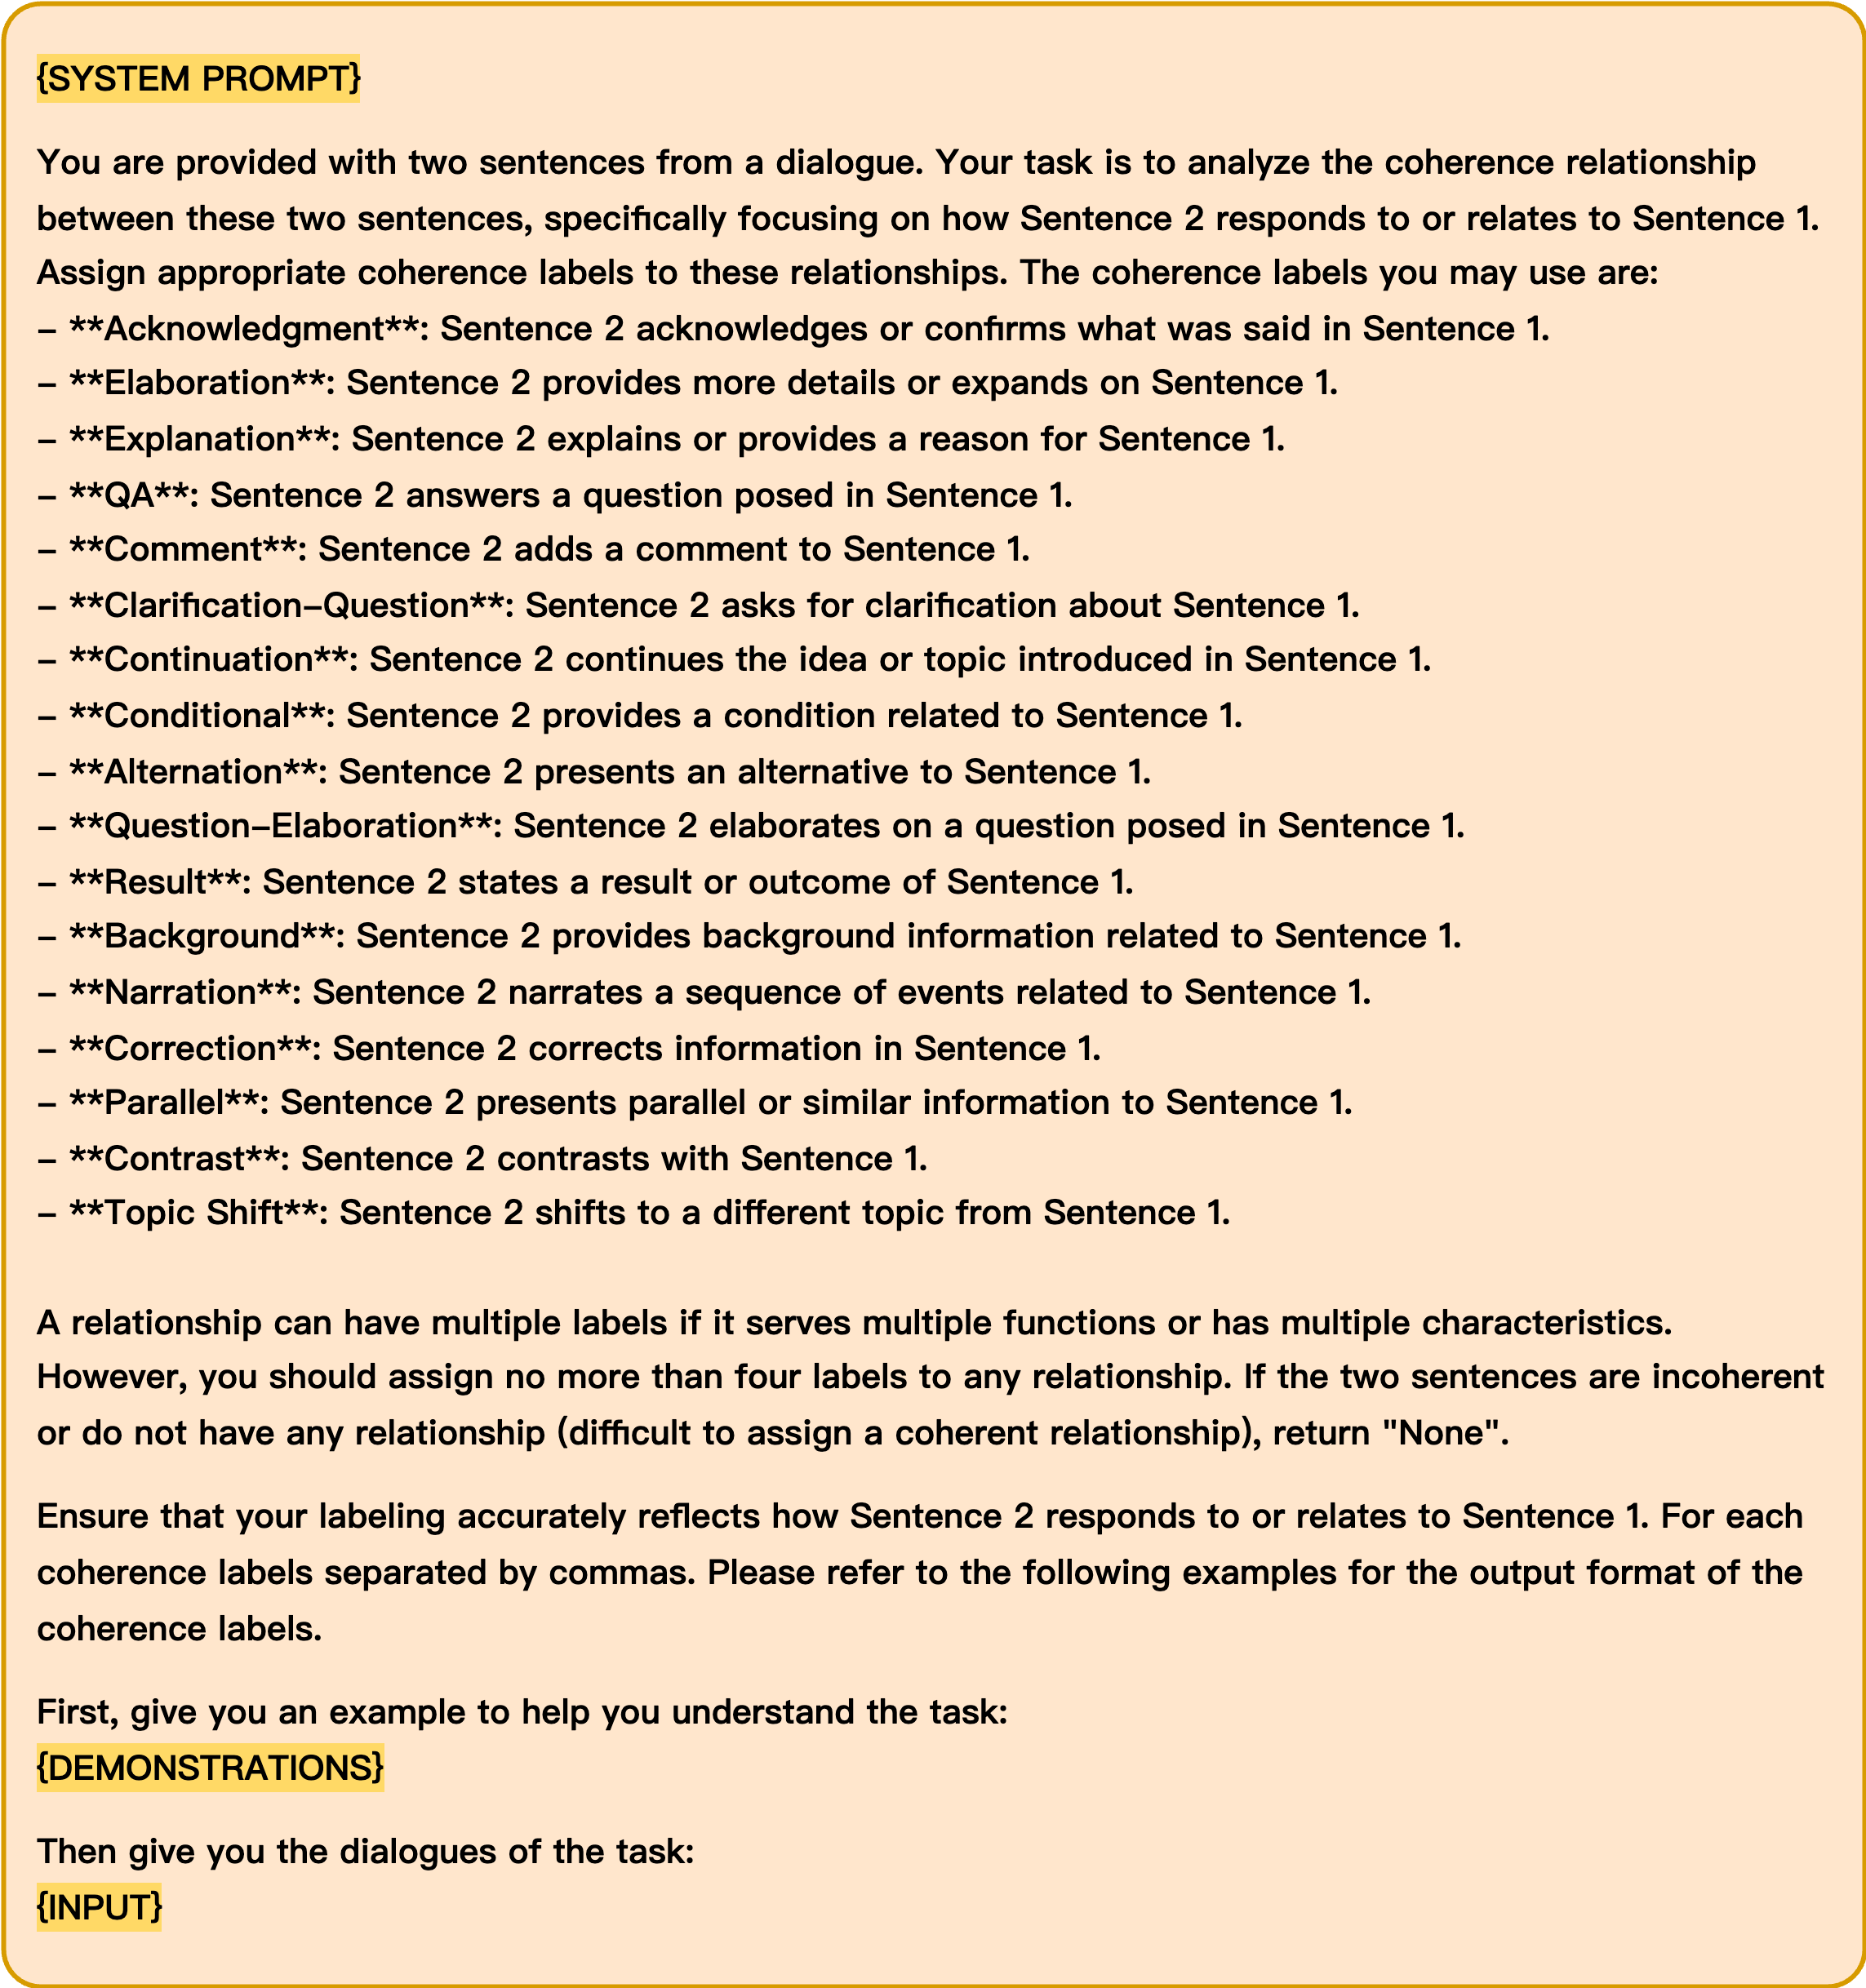
\includegraphics[width=0.5\textwidth]{./images/coherence_reltaions_annotated_prompt.png}
    \caption{The prompt of Coherence Relations Annotation.}
    \label{fig:coherence_reltaions_annotated_prompt}
\end{figure}

\subsection{Implementation Details}
The \textbf{MUDI} is mainly implemented in PyTorch. Our backbone Generator is BART-large\footnote[2]{https://huggingface.co/facebook/bart-large}. For Generator training, we train it using a batch size of 4 on 1 NVIDIA A100 80GB
GPU via the AdamW optimizer with a learning rate of \(5 \times 10^{-6}\) and a
weight decay of 0.01. For the Dialogue Graph Encoder training, it is conducted on a single NVIDIA RTX 4090 GPU using a batch size of 512. The training also employs the AdamW optimizer, but with a learning rate of \(2 \times 10^{-5}\) and the same weight decay of 0.01. In the Dialogue Graph Encoder, we initially employ the SBERT model "all-mpnet-base-v2"\footnote[3]{https://huggingface.co/sentence-transformers/all-mpnet-base-v2} to encode both the utterances and persona sentences, thereby initializing the node embeddings. We construct the Dialogue Graph by keeping the 3-hop neighbors. The model employs a 2-layer GNN with 4 multi-heads and a hidden dimension of 512. The weights for the different tasks are as follows: the weight of the Coherence Relation Classification task is 1.5, the weight of both types of Next Response Type Prediction tasks is 1.5, and the weight of the Link Prediction task is 1.2. For training the generator, we retain the most recent 5 turns of dialogue as historical context and choose the top-3 predicted response types for the prompt. We set \(\tau = 0.2\) for the Dynamic Weighted Aggregation.

% ----------------------------------------------
% Table 1: Text Similarity
% ----------------------------------------------

\begin{table*}
\centering
\def\arraystretch{1.3}%
\begin{tabular}{|c|c|c|c|c|c|c|}
\hline
\multicolumn{2}{|c|}{\multirow{2}{*}{\textbf{Model}}}  & \multicolumn{5}{c|}{\textbf{Text Similarity}} \\
\cline{3-7}

\multicolumn{2}{|c|}{} & BLEU-1 $\uparrow$ & BLEU-2 $\uparrow$ & ROUGE-1 $\uparrow$ & ROUGE-L $\uparrow$ & BERTScore $\uparrow$ \\
\hhline{|=======|}

\rowcolor[RGB]{242,164,100}
\multicolumn{7}{|c|}{\textbf{Large Language Model (Prompting)}} \\
\hhline{|=======|}

\multicolumn{2}{|c|}{\textbf{GPT-4}} &7.47 &2.40 &13.52 &11.06 &84.05 \\ 
\hhline{|=======|}

\rowcolor{yellow}
\multicolumn{7}{|c|}{\textbf{General Dialogue Generation}} \\
\hhline{|=======|}

\multicolumn{2}{|c|}{\textbf{DialoGPT}} &7.34	&1.54 &9.46 &8.41 &83.31 \\ 
\hline

\multirow{2}{*}{\textbf{PLATO}} & w/ persona &4.35	&1.01 &4.88 &4.80 &82.77 \\ 
\cline{2-7}

\multirow{2}{*}{\textbf{}} & w/o persona  &6.82 &1.86 &4.99 &4.77 &81.44 \\ 
\hhline{|=======|}

\rowcolor[RGB]{204,217,245}
\multicolumn{7}{|c|}{\textbf{Persona-based Dialogue Generation}} \\
\hhline{|=======|}

\multicolumn{2}{|c|}{\textbf{BoB}} &15.30 &5.39 &13.21 &12.48 &83.77 \\ 
\hline

% \multicolumn{2}{|c|}{\textbf{P$^{2}$BOT}} &- &- &- &- &- \\ 
% \hline

\multicolumn{2}{|c|}{\textbf{LMEDR}}		&15.47	&5.83	&13.28	&12.26	&85.00 \\ 
\hline

\multicolumn{2}{|c|}{\textbf{PAA}}          &\underline{16.55}    &6.28    &13.53 
&12.68    &84.42   \\
\hline

\multirow{3}{*}{\textbf{\begin{tabular}{@{}c@{}}MUDI \\ (ours)\end{tabular}}} &SP\textsubscript{$\tau=0.2$}	&15.14	&6.43	&14.87	&13.87	&85.07	\\
\cline{2-7}

\multirow{3}{*}{} &Emb\textsubscript{$\tau=0.2$}   &\underline{16.55}    &\underline{7.34}	&\textbf{\textcolor{red}{17.10}}	&\textbf{\textcolor{red}{16.13}}	&\underline{85.42}	\\
\cline{2-7}

\multirow{3}{*}{} &SP+Emb\textsubscript{$\tau=0.2$}   &\textbf{\textcolor{red}{18.19}} &\textbf{\textcolor{red}{7.77}}	&\underline{16.59}	&\underline{15.46}	&\textbf{\textcolor{red}{85.53}} \\
\hline
\end{tabular}
\caption{Automatic evaluation results on ConvAI2 dataset over our implemented approach. The best results in each column are in bold, while the second is underlined.}
\label{table:text-similarity}
\end{table*}

% ----------------------------------------------
% Table 2: Diversity
% ----------------------------------------------

\begin{table}[h]
\centering
\def\arraystretch{1.3}%
\begin{tabular}{|c|c|c|c|c|}
\hline
\multicolumn{2}{|c|}{\multirow{2}{*}{\textbf{Model}}}  &\multicolumn{3}{c|}{\textbf{Diversity}}\\
\cline{3-5}

\multicolumn{2}{|c|}{} &Ent-1 $\uparrow$ &Dist-1 $\uparrow$ &USR $\uparrow$ \\
\hhline{|=====|}

\rowcolor[RGB]{242,164,100}
\multicolumn{5}{|c|}{\textbf{Large Language Model (Prompting)}} \\
\hhline{|=====|}

\multicolumn{2}{|c|}{\textbf{GPT-4}} &9.40 &16.09 &1.00 \\ 
\hhline{|=====|}

\rowcolor{yellow}
\multicolumn{5}{|c|}{\textbf{General Dialogue Generation}} \\
\hhline{|=====|}

\multicolumn{2}{|c|}{\textbf{DialoGPT}} &\textbf{\textcolor{red}{9.05}} &36.84 &\underline{0.99} \\ 
\hline

\multirow{2}{*}{\textbf{PLATO}} & w/ persona &4.67 &\textbf{\textcolor{red}{58.18}} &0.61 \\ 
\cline{2-5}

\multirow{2}{*}{\textbf{}} & w/o persona &6.73 &43.34 &0.85 \\ 
\hhline{|=====|}

\rowcolor[RGB]{204,217,245}
\multicolumn{5}{|c|}{\textbf{Persona-based Dialogue Generation}} \\
\hhline{|=====|}


\multicolumn{2}{|c|}{\textbf{BoB}} &7.89 &41.75 &\underline{0.99} \\ 
\hline

% \multicolumn{2}{|c|}{\textbf{P$^{2}$BOT}} &- &- &- \\ 
% \hline

\multicolumn{2}{|c|}{\textbf{LMEDR}}  &7.14	&43.08	&0.94\\ 
\hline

\multicolumn{2}{|c|}{\textbf{PAA}}    &6.66	&40.27  &0.87 \\
\hline

\multirow{3}{*}{\textbf{\begin{tabular}{@{}c@{}}MUDI \\ (ours)\end{tabular}}} &SP\textsubscript{$\tau=0.2$}	&\underline{8.13}		&46.76	&\textbf{\textcolor{red}{1.00}}\\
\cline{2-5}

\multirow{3}{*}{} &Emb\textsubscript{$\tau=0.2$}   &7.65	&\underline{51.03}	&\textbf{\textcolor{red}{1.00}}\\
\cline{2-5}

\multirow{3}{*}{} &SP+Emb\textsubscript{$\tau=0.2$} 	&7.66	&47.68  &\textbf{\textcolor{red}{1.00}}\\
\hline
\end{tabular}
\caption{Automatic evaluation results for diversity tested on ConvAI2 dataset over our implemented approach. The best results in each column are in bold, while the second is underlined.}
\label{table:text-diversity}
\end{table}

% ----------------------------------------------
% Table 3: Coherence 
% ----------------------------------------------

\begin{table*}[h]
\centering
\def\arraystretch{1.3}%
\begin{tabular}{|c|c|c|c|c|}
\hline
\multicolumn{2}{|c|}{\multirow{2}{*}{\textbf{Model}}}  & \multicolumn{3}{c|}{\textbf{Coherence}} \\
\cline{3-5}

\multicolumn{2}{|c|}{} & QuantiDCE $\uparrow$ & DEAM $\uparrow$ & BARTScore$_{q \rightarrow r, c \rightarrow r}$ $\downarrow$ \\
\hline

\multicolumn{2}{|c|}{\textbf{GOLD}}          &3.19 / 2.83    &0.64 / 0.85    &5.74 / 5.70   \\
\hhline{|=====|}

\rowcolor[RGB]{242,164,100}
\multicolumn{5}{|c|}{\textbf{Large Language Model (Prompting)}} \\
\hhline{|=====|}

\multicolumn{2}{|c|}{\textbf{GPT-4}} &3.41 / 2.92 &0.87 / 0.96 &4.24 / 3.73 \\ 
\hhline{|=====|}

\rowcolor{yellow}
\multicolumn{5}{|c|}{\textbf{General Dialogue Generation}} \\
\hhline{|=====|}

\multicolumn{2}{|c|}{\textbf{DialoGPT}} &\textbf{\textcolor{red}{3.23}} / 2.79 &\textbf{\textcolor{red}{0.70}} / \textbf{\textcolor{red}{0.88}} &5.12 / 5.19 \\ 
\hline

% \multirow{2}{*}{\textbf{PLATO}} & w/ persona &3.32 / 3.43	&0.22 / 0.75 &6.42 / 6.63 \\ 
\multirow{2}{*}{\textbf{PLATO}} & w/ persona &1.68 / 1.57	&0.22 / 0.75 &6.42 / 6.63 \\ 
\cline{2-5}

\multirow{2}{*}{\textbf{}} & w/o persona  &1.87 / 1.77 &0.25 / 0.74 &5.83 / 5.80 \\ 
\hhline{|=====|}

\rowcolor[RGB]{204,217,245}
\multicolumn{5}{|c|}{\textbf{Persona-based Dialogue Generation}} \\
\hhline{|=====|}

\multicolumn{2}{|c|}{\textbf{BoB}} &2.99 / 2.76 &0.39 / 0.86 &5.82 / 5.92 \\ 
\hline

% \multicolumn{2}{|c|}{\textbf{P$^{2}$BOT}} &- &- &- \\ 
% \hline

\multicolumn{2}{|c|}{\textbf{LMEDR}}		&2.89 / 2.90	&0.43 / 0.78	&5.32 / 4.99  \\ 
\hline

\multicolumn{2}{|c|}{\textbf{PAA}}           &2.70 / \underline{2.93}    &0.56 / 0.83    &5.17 / \underline{4.62}   \\
\hline

\multirow{3}{*}{\textbf{\begin{tabular}{@{}c@{}}MUDI \\ (ours)\end{tabular}}} &SP\textsubscript{$\tau=0.2$}	&3.05 / 2.84	&0.63 / 0.85	&\underline{4.67} / \textbf{\textcolor{red}{4.61}}	\\
\cline{2-5}

\multirow{3}{*}{} &Emb\textsubscript{$\tau=0.2$}   &\textbf{\textcolor{red}{3.23}} / \textbf{\textcolor{red}{2.94}}    &0.56 / 0.82	&4.80 / 4.83 \\
\cline{2-5}

\multirow{3}{*}{} &SP+Emb\textsubscript{$\tau=0.2$}   &\underline{3.21} / 2.92	&\underline{0.64} / \underline{0.86}	&\textbf{\textcolor{red}{4.66}} / 4.66	\\
\hline
\end{tabular}
\caption{Automatic evaluation results for coherence tested on the ConvAI2 dataset. The best results in each column are in bold, while the second-best results are underlined. The score on the left considers only the local coherence between the query and the response, while the score on the right takes into account the global coherence between the entire dialogue and the response.}
\label{table:coherence}
\end{table*}

% ----------------------------------------------
% Table 4: Personalization & Feature Coverage
% ----------------------------------------------

\begin{table*}[h]
\centering
\def\arraystretch{1.3}%
\begin{tabular}{|c|c|c|c|c|c|}
\hline
\multicolumn{2}{|c|}{\multirow{2}{*}{\textbf{Model}}}  &\multicolumn{2}{c|}{\textbf{Personalization}} &\multicolumn{2}{c|}{\textbf{Feature Coverage}}\\
\cline{3-6}

\multicolumn{2}{|c|}{} &C.Score $\uparrow$ &BARTScore$_{p \leftrightarrow r}$ $\downarrow$ &FCR$_{q}$ $\uparrow$ &FCR$_{p}$ $\uparrow$ \\
\hline

\multicolumn{2}{|c|}{\textbf{GOLD}}      &4.10   &5.68 &7.69 &4.52 / 3.60\\
\hhline{|======|}

\rowcolor[RGB]{242,164,100}
\multicolumn{6}{|c|}{\textbf{Large Language Model (Prompting)}} \\
\hhline{|======|}

\multicolumn{2}{|c|}{\textbf{GPT-4}} &2.86 &4.06 &6.95 &3.60 \\ 
\hhline{|======|}

\rowcolor{yellow}
\multicolumn{6}{|c|}{\textbf{General Dialogue Generation}} \\
\hhline{|======|}

\multicolumn{2}{|c|}{\textbf{DialoGPT}} &4.53 &5.39 &\textbf{\textcolor{red}{6.78}} &4.45  \\ 
\hline

\multirow{2}{*}{\textbf{PLATO}} & w/ persona &0.56 &6.06 &1.20 &0.92 \\ 
\cline{2-6}

\multirow{2}{*}{\textbf{}} & w/o persona  &0.18 &5.83 &3.23 &0.28 \\ 
\hhline{|======|}

\rowcolor[RGB]{204,217,245}
\multicolumn{6}{|c|}{\textbf{Persona-based Dialogue Generation}} \\
\hhline{|======|}

\multicolumn{2}{|c|}{\textbf{BoB}} &0.51 &5.52 &3.68 &0.42  \\ 
\hline

% \multicolumn{2}{|c|}{\textbf{P$^{2}$BOT}} &- &- &- &-  \\ 
% \hline

\multicolumn{2}{|c|}{\textbf{LMEDR}}		&7.38	&5.27 &4.63	 &6.99 \\ 
\hline


\multicolumn{2}{|c|}{\textbf{PAA}}       &\textbf{\textcolor{red}{15.19}}   &\textbf{\textcolor{red}{4.26}} &\underline{4.66}    &\textbf{\textcolor{red}{13.84}} \\
\hline

\multirow{3}{*}{\textbf{\begin{tabular}{@{}c@{}}MUDI \\ (ours)\end{tabular}}} &SP\textsubscript{$\tau=0.2$}	&\underline{11.87} &\underline{4.53} &\underline{4.66} &6.50	\\
\cline{2-6}

\multirow{3}{*}{} &Emb\textsubscript{$\tau=0.2$}   &9.70	&4.75 &4.36 &\underline{7.77} \\
\cline{2-6}

\multirow{3}{*}{} &SP+Emb\textsubscript{$\tau=0.2$}  &9.75	&4.76 &4.05 &5.01 \\
\hline
\end{tabular}
\caption{Automatic evaluation results for personalization and feature coverage tested on the  ConvAI2 dataset. The best results in each column are in bold, while the second-best results are underlined.}
\label{table:personalization}
\end{table*}

\subsection{Prompt Structure for LLM Prompting in Evaluation}
The prompt used for GPT-4 can be seen in Figure \ref{fig:llm_inference_prompt}.

\begin{figure}[ht]
    \centering
    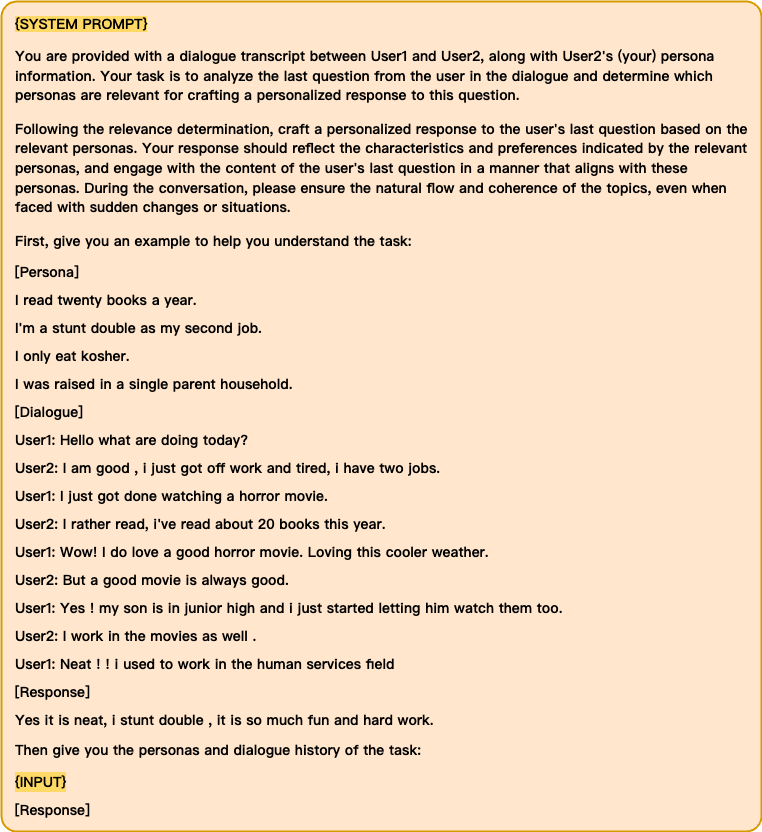
\includegraphics[width=0.5\textwidth]{./images/llm_inference_prompt.png}
    \caption{The prompt of LLM inference on Personalized Dialogue Generation task.}
    \label{fig:llm_inference_prompt}
\end{figure}

\subsection{Automatic Metrics}

More specifically, aside from the evaluation metrics discussed in the Experiments chapter, we assess the quality of dialogue responses from four perspectives: 

(1) \textbf{Text-similarity}: To evaluate the similarity between the generated responses and the ground-truth responses, we employ BLEU \cite{papineni-etal-2002-bleu} and ROUGE \cite{lin-2004-rouge} metrics, which focus on the word overlap level. Additionally, we utilize BERTScore \cite{zhang-etal-2020-bert-score}, which measures the semantic similarity between generated responses and ground-truth using contextual embeddings from BERT. This helps capture nuances that traditional overlap-based metrics might miss.

(2) \textbf{Diversity}: We assess the diversity and informativeness of the generated responses at token, sentence, and corpus levels. We utilize Distinct-n (Dist-$n$) metrics \cite{li-etal-2016-diversity} to measure the proportion of unique n-grams (n=1) relative to the total number of n-grams in the generated responses. Additionally, we employ Entropy-n (Ent-$n$) \cite{zhang-etal-2018-generating} to evaluate the uncertainty or randomness of the distribution of n-grams (n=1) in the generated text. We also calculate the Unique Sentence Ratio (USR) \cite{li-etal-2020-generate}, which quantifies text diversity by measuring the proportion of unique sentences among all predicted responses.

(3) \textbf{Coherence}: Previous studies often omit explicit evaluations of Coherence, assuming that Fluency can also measure the coherence of dialogues. However, this approach does not directly account for the coherence of generated responses with the context and query, an aspect often presumed to be covered by fluency. To measure this unexplored dimension, our research incorporates specific coherence metrics to provide a more accurate and holistic assessment of response quality. Specifically, We employ several metrics. Firstly, we use QuantiDCE \cite{ye-etal-2021-towards-quantifiable} and DEAM \cite{ghazarian-etal-2022-deam}, which are state-of-the-art metrics in dialogue coherence evaluation. These metrics assess both how logically the responses align with the preceding query or the entire context within the dialogue, and how well the utterances in a conversation are unified, leading to a consistent and coherent interaction. Additionally, we utilize BARTScore \cite{yuan-etal-2021-bartscore} to measure coherence under the faithfulness setting discussed in the paper.

(4) \textbf{Personalization}: To assess the personalization of the generated responses, we first measure the alignment between the persona and responses. First, we apply Consistency Score (C.Score) \cite{madotto-etal-2019-personalizing}, which leverages a NLI model to predict consistency between response and persona. Additionally, we utilize the BARTScore \cite{yuan-etal-2021-bartscore}, which provides a method to calculate the semantic overlaps between texts. Specifically, we compute: (a) Precision (persona → response): This measures how closely the generated responses adhere to the input persona, reflecting the degree to which the model captures persona-specific attributes in the response. (b) Recall (response → persona): This assesses whether all aspects of the persona are sufficiently covered by the responses, indicating the comprehensiveness of the persona information in the generated text. we report the F1 Score is then calculated from these Precision and Recall scores to provide a balanced measure of personalization, capturing both the accuracy and completeness of the generated responses in reflecting the specified persona.

Moreover, to better assess whether the generated responses accurately incorporate important features from the persona or the query, we utilize Large Language Models (LLMs)\footnote[4]{https://huggingface.co/meta-llama/Meta-Llama-3-70B-Instruct} to identify key terms (features) from these persona descriptions or dialogue utterances. We then employ a NLI model to calculate the Feature Coverage Ratio (FCR), ensuring that critical features are effectively represented in the responses. The example of the feature-annotated table mentioned earlier is shown in Table \ref{table:fcr-feature-annotated-example}.

\subsection{Main Results}

Apart from DialoGPT, we use the context of the most recent 5 turns as dialogue history. After testing, we found that DialoGPT starts to talk nonsense when given more than 2 turns of context. Therefore, for DialoGPT, we only use the most recent 2 turns.

In Table \ref{table:text-similarity}, we report experimental results on Text Similarity evaluation. Our method offers better BLEU, ROUGE, and BERTScore compared with baseline methods. Specifically, MUDI's BLEU-1, ROUGE-1, and ROUGE-L scores reach 18.19, 17.10, and 16.13, respectively, outperforming existing methods by 1.64, 3.57, and 3.45. As shown in Table \ref{table:text-diversity}, we report the Diversity evaluation. MUDI's USR is 1.0, indicating that it can generate completely unique responses under different queries and personas. Additionally, we achieved the second-highest scores in Ent-1 and Dist-1. Upon examining the outputs from PLATO, we found that they often generate shorter sentences, such as 'me to!!'. Shorter sentences tend to inflate certain metrics, like Dist-1, because they typically involve less repetition of words within a single response, leading to high distinct scores. This suggests that while our method ranks second, it could provide more substantial and contextually rich responses compared to PLATO. Furthermore, our approach achieves the highest scores among all Persona-based dialogue generation methods and significantly surpasses other baselines in Dist-1, outperforming them by 7.95. This performance establishes our method could generate varied and engaging responses.

In addition, Table \ref{table:coherence} presents the results of the Coherence evaluation. Compared to other persona-based methods, MUDI has made significant progress in QuantiDCE, DEAM, and BARTScore, particularly in assessing the coherence between the query and response (left-side scores). This indicates that our approach indeed enables the model to generate responses with enhanced local coherence. Furthermore, MUDI also achieves excellent results in global coherence, which evaluates the coherence between the entire dialogue context and the response (right-side scores).

Finally, Table \ref{table:personalization} presents the results of evaluating Personalization and Feature Coverage. PAA significantly outperforms other methods in scores for Personalization and FCR$_p$. Upon further examination, we discovered that this is because PAA frequently generates sentences that are exact restatements of the persona description, often ignoring the relevance to the query. As a result, its high scores in Personalization can be attributed to this tendency. Excluding the special case of PAA, MUDI achieves excellent results in Personalization compared to other methods. Combined with the previously discussed results from the Coherence evaluation (Table \ref{table:personalization}), this demonstrates that our approach successfully balances discourse relations and persona. It generates responses that effectively consider both aspects simultaneously. Furthermore, our model achieves comparable scores in the Coherence evaluation compared to DialoGPT, which focuses on general dialogue generation.

In evaluating powerful LLMs like GPT-4, we find that they excel at generating lengthy responses and maintaining coherence between questions and dialogue context. Consequently, GPT-4 stands out in Coherence evaluation, scores highly in Ent-1, and performs well in FCR$_q$. However, this also results in a lower overlap with the ground-truth responses, leading to lower Text Similarity scores. Moreover, the longer sentences generated lead to a lower Dist-1 score. Another observation is that GPT-4 performs poorly in evaluations related to Personalization and FCR$_p$. This indicates that although existing LLMs are powerful and adept at generating fluent sentences, tasks such as personalized dialogue generation require deeper understanding and inferential capabilities, areas in which they currently fall short.

In summary, compared to existing methods, our approach MUDI not only significantly improves performance in Text Similarity scores but also excels at integrating discourse relations and persona information. This enables us to generate personalized responses that are not only rich in content and diverse but also encompass these aspects. Moreover, in Coherence evaluations, our method achieves scores comparable to those of state-of-the-art models specialized in open-domain dialogue generation.

\subsection{Analysis}

\subsubsection{The Effect of Dialogue Graph Encoder}
We analyze the effectiveness of the Dialogue Graph Encoder (discussed in Section 3.2.2 fine-tuning phase) under various settings. (1) \textbf{Context+Persona (Attention)}: This is our primary method where we utilize an Attention-based Feature Fusion approach to integrate representations from both the Dialogue Graph and the Persona Graph. (2) \textbf{Context+Persona (Add)}: We replace the Attention-based Feature Fusion approach with a simple addition of the persona and context representations. (3) \textbf{Context}: In this setting, we solely rely on the representation from the Dialogue Graph. (4) \textbf{Persona}: Here, we use only the representation from the Persona Graph. (5) \textbf{Random}: A random vector replaces the output of the Dialogue Graph Encoder. (6) \textbf{None}: The Dialogue Graph Encoder is completely removed from the process, allowing the generator to receive only the context and persona information from the Text Encoder. The comprehensive experimental results can be found in Figure \ref{fig:effectiveness_of_dialogue_graph_encoder}. We report the metrics for BLEU-1, ROUGE-1, and Consistency Score (C.Score).

\begin{figure}[ht]
    \centering
    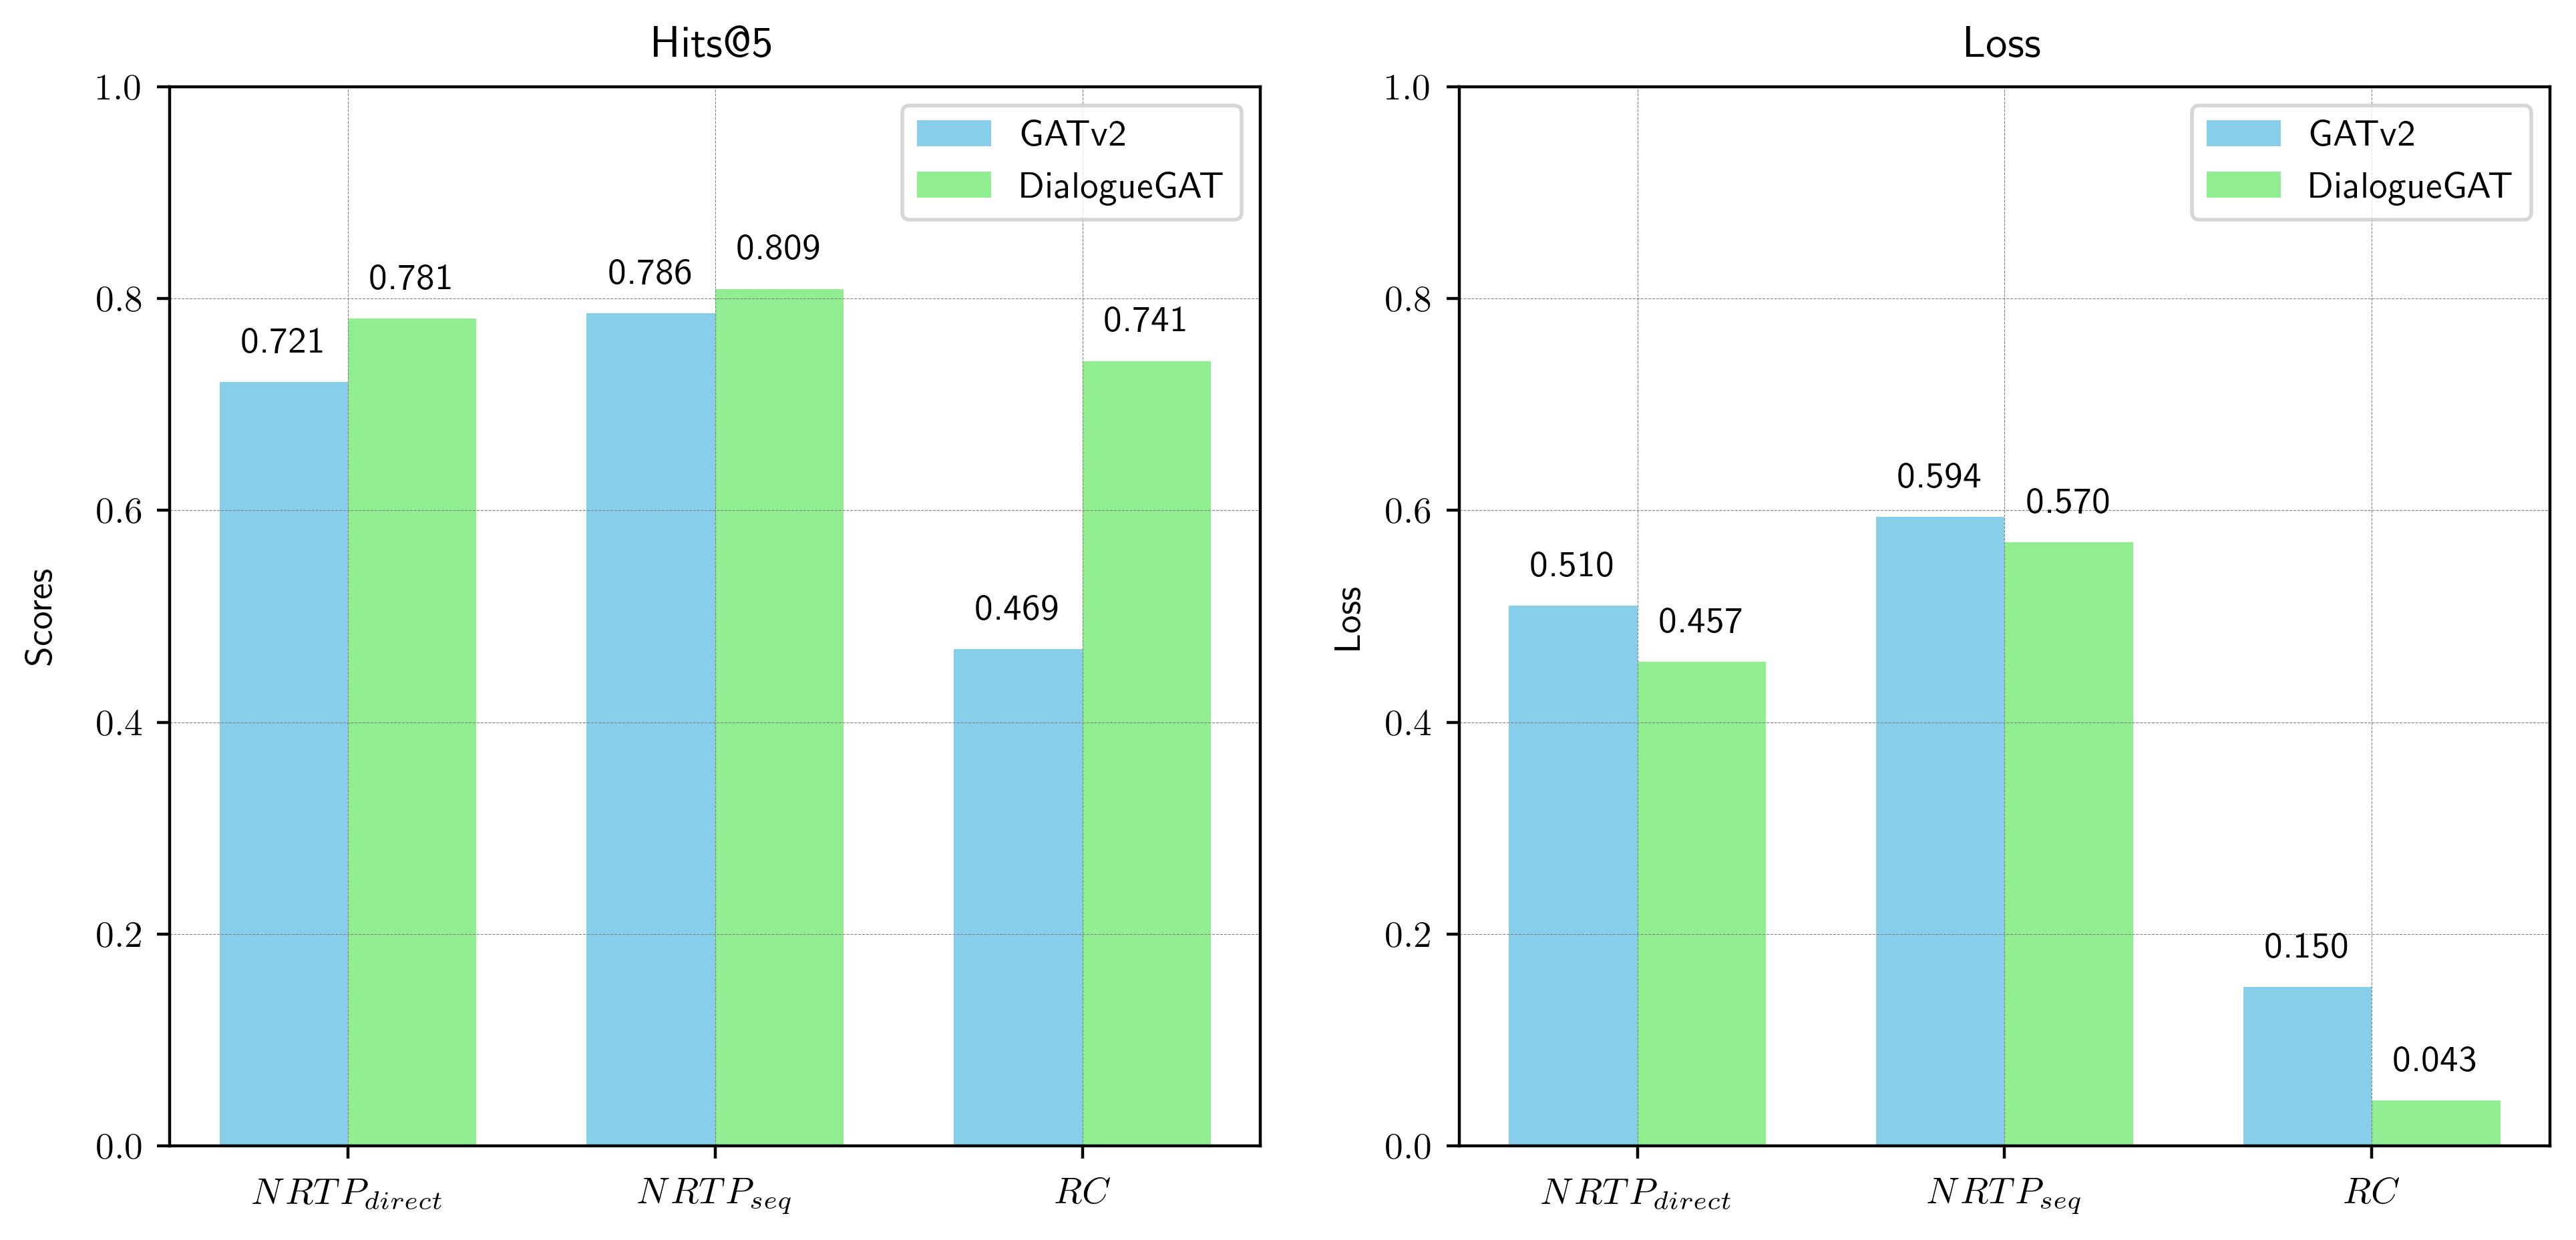
\includegraphics[width=0.5\textwidth]{./images/compare_gatv2_dialoguegat.png}
    \caption{Comparison of GATv2 and DialogueGAT (our proposed) as Dialogue Graph Encoders in Different Tasks. \textit{NRTP} denotes Next Response Type Prediction; \textit{RC} denotes Relations Classification.}
    \label{fig:compare_gatv2_dialoguegat}
\end{figure}

Our experimental results demonstrate that the attention-based feature fusion approach (Context+Persona (Attention)) significantly outperforms other methods in terms of BLEU-1 and ROUGE-1 scores. These findings confirm that effectively integrating contextual and persona information through an attention mechanism enhances the similarity of the generated responses to the ground-truth responses. In contrast, simpler methods such as addition (Context+Persona (Add)) or those relying solely on context or persona information exhibit lower performance. The scores drastically decrease when random vectors are employed or when the dialogue graph encoder is omitted entirely, which emphasizes the crucial role of structured and meaningful input in producing coherent responses. The consistency scores further elucidate the models' ability to generate responses that align with persona traits. The superior performance of the attention-based method suggests its effectiveness in maintaining persona consistency within the responses. Notably, employing random vectors results in negative C.Score values, indicating that some generated responses are not only irrelevant but also contradictory to the defined personas.

These outcomes reinforce the importance of utilizing attention-based feature fusion in dialogue systems, especially in tasks that require a nuanced understanding of both context and persona. Additionally, the inferior results associated with random inputs and the complete removal of the dialogue graph encoder highlight potential risks of response incoherence and contradiction when inputs are not integrated thoughtfully. We present examples of generated results for these settings in Table \ref{table:case_study_effectiveness_of_dialogue_graph_encoder}.

\begin{figure}[h]
    \centering
    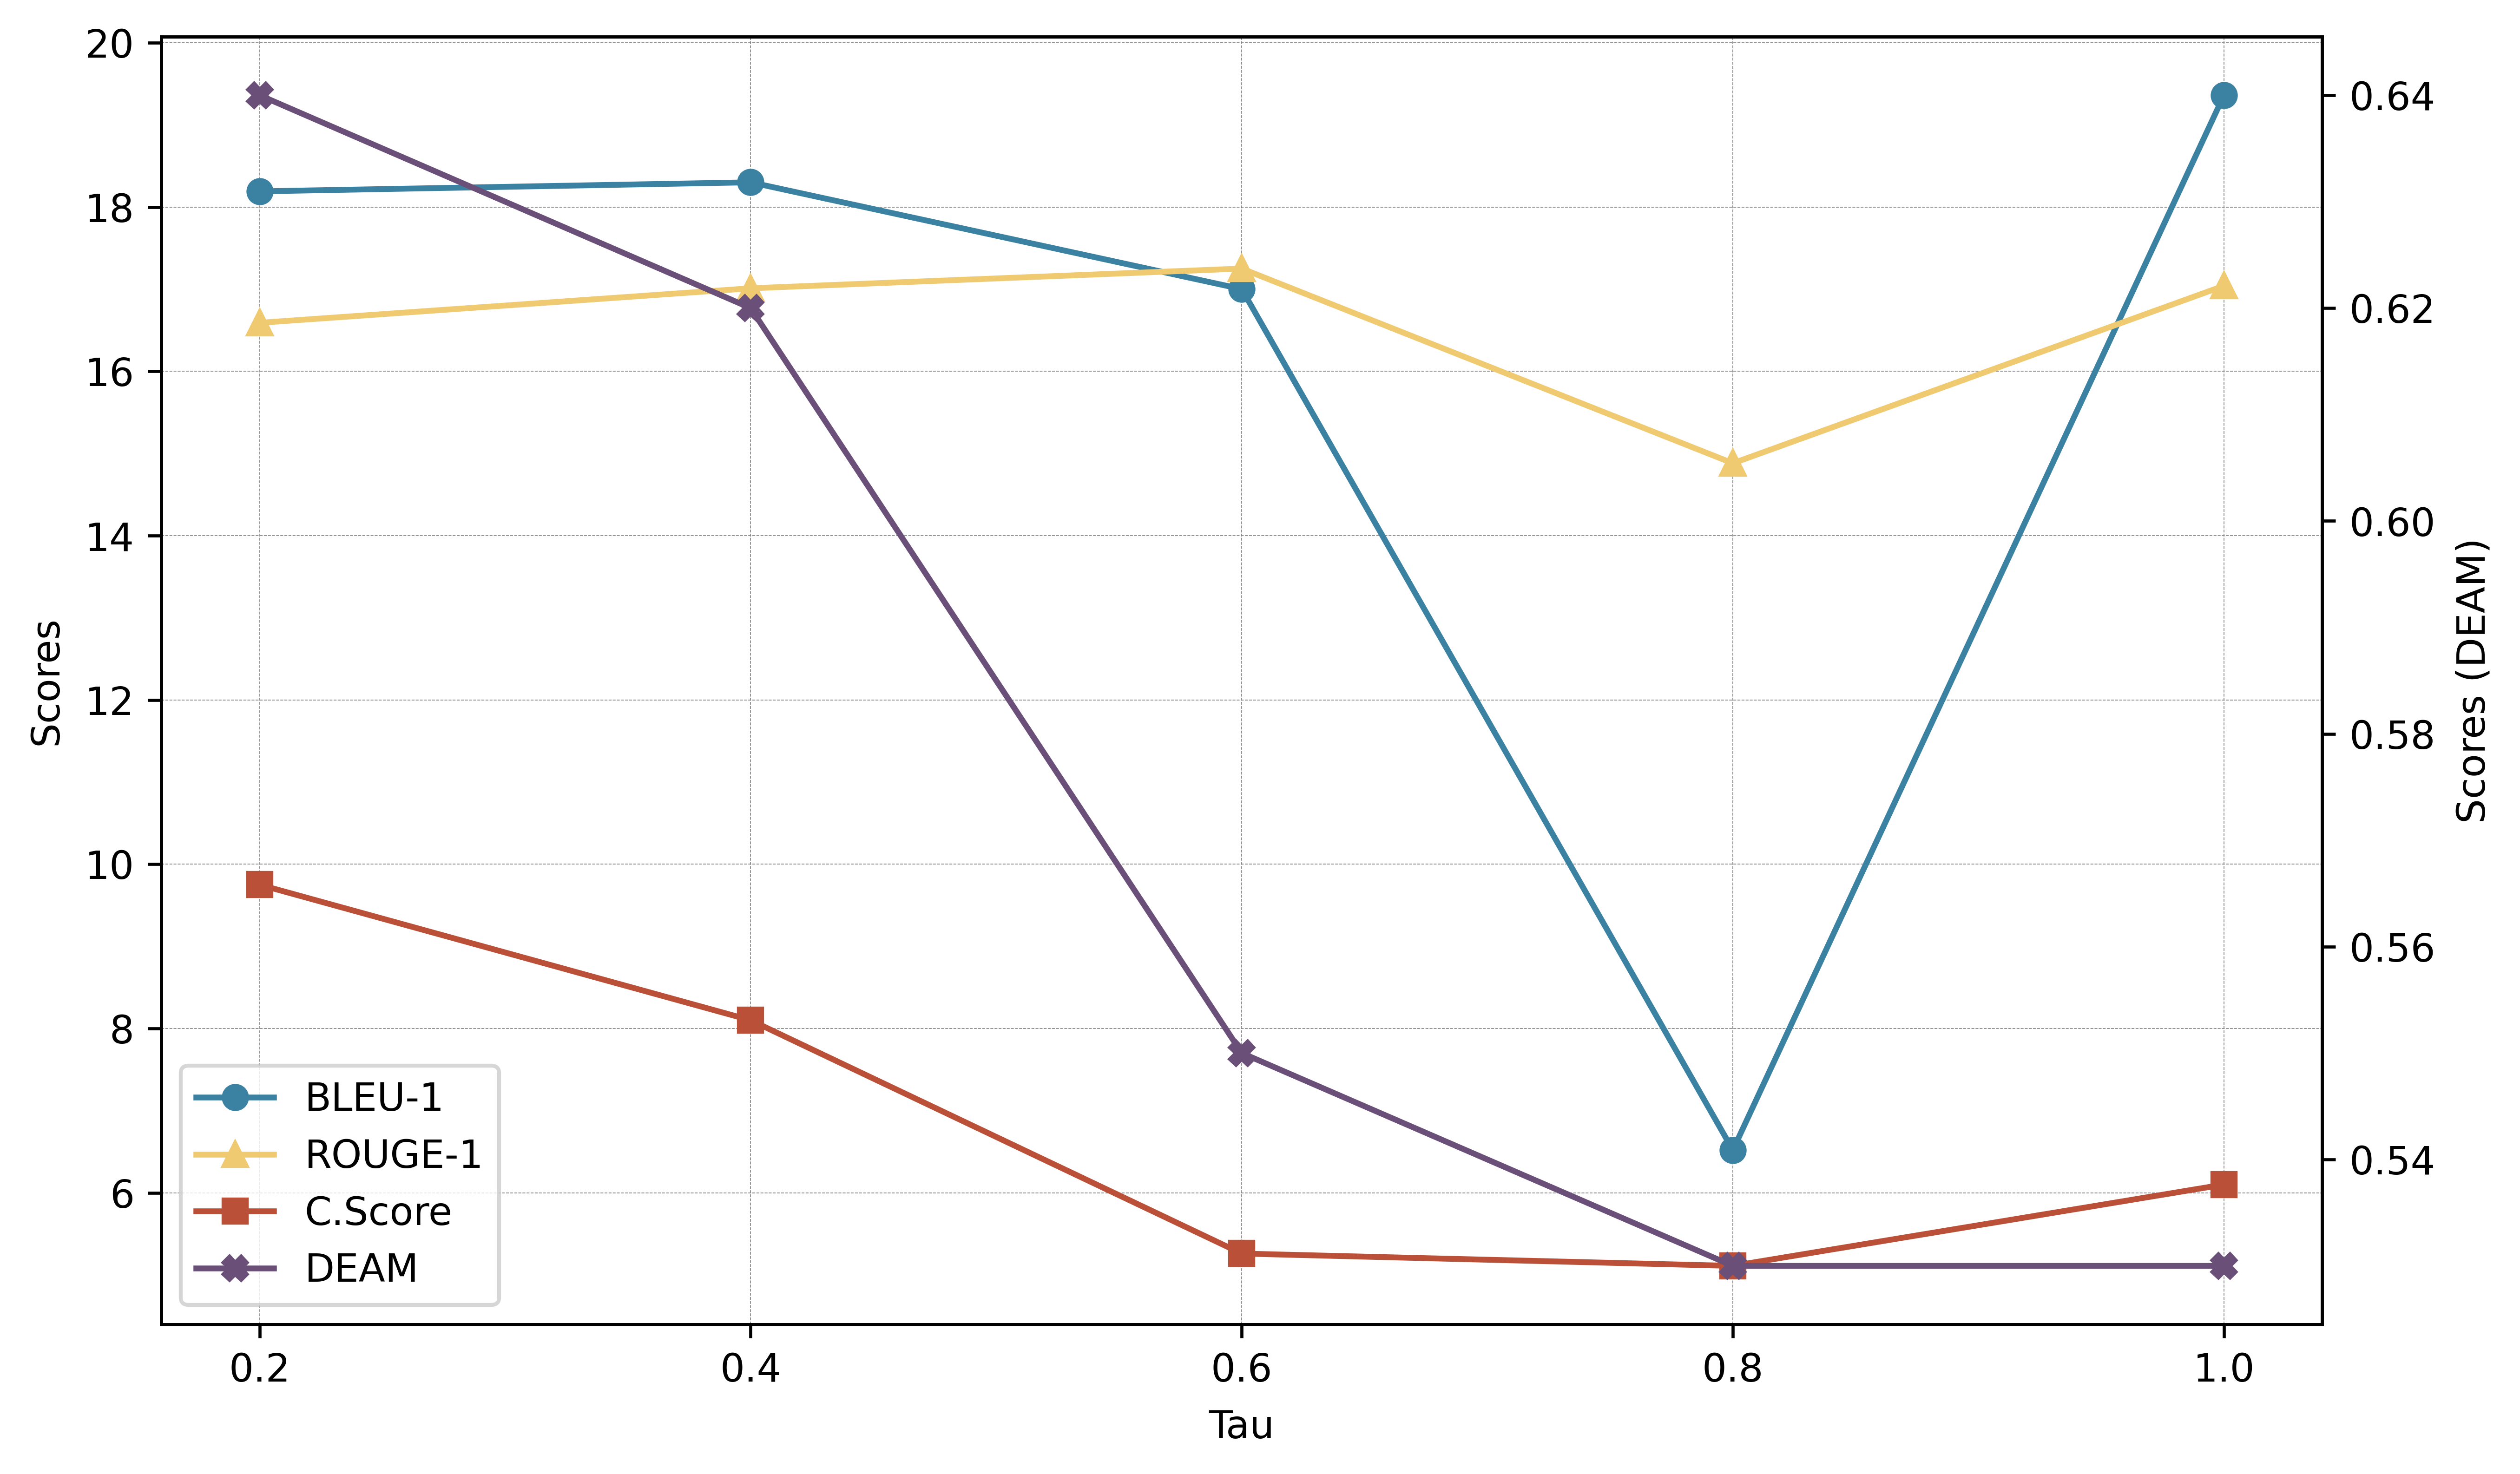
\includegraphics[width=0.5\textwidth]{./images/effectiveness_of_tau_with_deam.png}
    \caption{Performance analysis of $\tau$ in Dynamic Weighted Aggregation.}
    \label{fig:effectiveness_of_tau}
\end{figure}

\subsubsection{The Effect of Tau Values in Dynamic Weighted Aggregation}

We analyze the effectiveness of $\tau$ in Dynamic Weighted Aggregation (discussed in Section 3.4). According to our results, shown in Figure \ref{fig:effectiveness_of_tau}, the scores gradually decrease as $\tau$ increases, with the most significant drop occurring at 0.8. Additionally, we observed that the scores, particularly for BLEU-1, actually increase when $\tau$ reaches 1.0. We hypothesize that this is due to our approach, which involves a residual connection (Eq. \ref{eq:dynamic_weighted_aggregation_output}) between the outputs of the Text Encoder and the Dialogue Graph Encoder with the results of the dynamic weighting. When $\tau$ is set to 1.0, it effectively considers only the original outputs, thus retaining a certain level of generative capability. However, this does not enhance persona consistency as much as when $\tau$ is optimally adjusted. This observation confirms that through Dynamic Weighted Aggregation, we can appropriately balance discourse and persona information.


\begin{table*}[ht]
\centering
\def\arraystretch{1.2}%
\begin{tabular}{|p{3.5cm}|p{12cm}|}

\hline
\rowcolor{yellow}
\multicolumn{2}{|c|}{\textbf{Persona}} \\
\hline
\multicolumn{2}{|l|}{I have two dogs.} \\
\multicolumn{2}{|l|}{I like to work on vintage cars.} \\
\multicolumn{2}{|l|}{My favorite music is country.} \\
\multicolumn{2}{|l|}{I own two vintage mustangs.} \\
\hline

\rowcolor{yellow}
\multicolumn{2}{|c|}{\textbf{Context}} \\
\hline
\multicolumn{2}{|l|}{Q: Hi! How are you doing tonight?} \\
\multicolumn{2}{|l|}{R: I'm doing great. Just relaxing with my two dogs.} \\
\multicolumn{2}{|l|}{Q: Great. In my spare time I do volunteer work.} \\
\multicolumn{2}{|l|}{R: That's neat. What kind of volunteer work do you do?} \\
\multicolumn{2}{|l|}{Q: I work in a homeless shelter in my town.} \\
\multicolumn{2}{|l|}{R: Good for you. Do you like vintage cars? I've two older mustangs.} \\
\multicolumn{2}{|l|}{Q: Cool. Not really into cars. My day job is wrestling.} \\
\multicolumn{2}{|l|}{R: Cars are my thing. Vintage cars. I love working on them. Wrestling? Do you enjoy it?} \\
\multicolumn{2}{|l|}{Q: Yes, I love the crowds, getting to know people.} \\
\multicolumn{2}{|l|}{R: I didn't think about the crowd aspect of wrestling. I do not like crowds.} \\
\multicolumn{2}{|l|}{Q: Understood. When I need to be alone, I work out a few times each week.} \\
\multicolumn{2}{|l|}{R: I agree. Working out is a great way to burn off steam. Do you like country music?} \\
\hline

\rowcolor{yellow}
\multicolumn{2}{|c|}{\textbf{Query}} \\
\hline
\multicolumn{2}{|l|}{A little bit. I can get into taylor swift.} \\

\hhline{|==|}
\rowcolor[RGB]{204,217,245}
\multicolumn{2}{|c|}{\textbf{Response}} \\
\hhline{|==|}
\textbf{Context+Persona (Attention)} & I do not like her. She's a bit too uptight for my taste. But I like her music. \\
\textbf{Context+Persona (Add)} & I can get may may and m and may and j on for more of her \\
\textbf{Context} &  What was she like? \\
\textbf{Persona} & I like country music too. \\
\textbf{Random} & you The A’ A A played The old White lead A Barbara at The The 17… \\
\textbf{None} & I like country music as well. \\

\hline
\end{tabular}
\caption{Case analysis of the effectiveness of Dialogue Graph Encoder.}
\label{table:case_study_effectiveness_of_dialogue_graph_encoder}
\end{table*}

\subsubsection{Ablation Study}
In our approach, to enable the dialogue graph encoder to understand the dialogue structure and adapt to subsequent coherence-related fine-tuning tasks, we designed several pre-training tasks aimed at capturing the dialogue structure. Therefore, we conducted an ablation study on these tasks to examine their impact on generating personalized responses later on. We present the results for three important metrics, coherence, personalization, and diversity, to demonstrate the impact of the pretraining task on the generated outcomes.
The results of this ablation study are shown in Table \ref{table:ablation_study_pretraining}, we observed that first, after removing the Shortest Path Prediction task, the scores for local coherence (left side of the QuantiDCE score), persona-consistency (C.Score), and diversity (Dist-1) began to drop sharply. The goal of the Turn Classification task is to help the model capture the local structure. When this task was removed, there was a dramatic decline in scores for local coherence and persona-consistency, proving that this task aids the model in effectively capturing semantic similarities in dialogue data. Furthermore, if the Graph Reconstruction task is removed, there is a continuing downward trend in personalization scores. This confirms that our three self-supervised pretraining tasks are beneficial for the model’s understanding of dialogue structure and assist in coherence-related fine-tuning tasks, ultimately impacting the model's ability to balance coherence and persona information when generating personalized responses.

\begin{table}[H]
    \centering
    \def\arraystretch{1.3}%
    \begin{tabular}{crrr}
    \hline
          Models & QuantiDCE & C.Score & Dist-1 \\
          \hline
          \textbf{MUDI}_{\text{SP}}  & 3.05 / 2.84 & 11.87 & 46.76 \\
         \hspace*{0.7cm} w/o SPP & 2.72 / 2.92  & 7.05 & 34.07  \\
         \hspace*{0.5cm} w/o TC  & 2.69 / 2.89  & 1.18 & 33.07 \\
         \hspace*{0.5cm} w/o GR & 2.72 / 2.92  & 6.49 & 33.94 \\
    \hline
    \end{tabular}
    \caption{Ablation study of the Dialogue Graph Encoder for pre-training tasks.}
    \label{table:ablation_study_pretraining}
\end{table}

\subsection{Case Study}
Teable \ref{table:case_study_1}, \ref{table:case_study_2}, \ref{table:case_study_3}, and \ref{table:case_study_4} present the personalized responses generated by various methods using the ConvAI2 dataset. The responses generated by the proposed method, \textbf{MUDI}, demonstrated greater consistency with their respective personas and showed higher coherence with both the context and the query, appearing more human-like. As illustrated in Table \ref{table:case_study_1}, the responses from BoB were incoherent with the query, though they remained consistent with the persona. PAA often overfocused on the persona, leading to repetitive narratives of the persona description. Both LMEDR and our model produced responses that were more coherent, basing them on the user persona, but MUDI was able to generate more detailed replies, such as adding personal aspirations to the basic response about family support. 

In Table \ref{table:case_study_2}, the responses generated by BoB were irrelevant to the personas and incoherent with the context. PAA exhibited a global incoherence from the dialogue context, failing to maintain a logical flow in the conversation. While LMEDR generated a somewhat relevant response indicating a dream car, it lacked depth and personal context. On the other hand, MUDI produced a more personalized and contextually rich response that not only mentions the dream car but also integrates family dynamics, demonstrating a deeper understanding of the persona's background and the complexities in their personal relationships. 

In Table \ref{table:case_study_3}, BoB and PAA tended to overlook content from the ongoing dialogue, generating repetitive responses that rendered the entire conversation incoherent. Although LMEDR was able to generate adequate responses, our model excelled by producing more natural responses through the inclusion of responsive questions. 

As shown in Table \ref{table:case_study_4}, BoB diverged from the persona's preference by mentioning classic rock instead of country music, showing a misalignment with the user’s interests. LMEDR and PAA both correctly identified and responded with a generic appreciation for country music, aligning with the persona’s interests, yet their responses lacked specific engagement with the user’s mention of Taylor Swift or deeper personal nuances. MUDI's response, while initially not favoring Taylor Swift, cleverly circled back to acknowledge her music, demonstrating not only a nuanced understanding of the persona's tastes but also adding an interesting twist to the conversation. This illustrates MUDI's ability to generate engaging and lifelike responses, making the interaction more intriguing for users.

In summary, our model \textbf{MUDI} effectively combines dialogue and persona elements to generate appropriate responses. Furthermore, it excels at using responsive questions to enhance the conversation's naturalness.


% ----------------------------------------------
% Case Study 1
% ----------------------------------------------

\begin{table*}[ht]
\centering
\def\arraystretch{1.2}%
\begin{tabular}{|l|p{11cm}|}

\hline
\rowcolor{yellow}
\multicolumn{2}{|c|}{\textbf{Persona}} \\
\hline
\multicolumn{2}{|l|}{My dream car is a rolls royce ghost.} \\
\multicolumn{2}{|l|}{I currently work for a watch dealer.} \\
\multicolumn{2}{|l|}{My family does not support my career choices.} \\
\multicolumn{2}{|l|}{I often shop for shoes and watches.} \\
\multicolumn{2}{|l|}{I like shopping.} \\
\hline

\rowcolor{yellow}
\multicolumn{2}{|c|}{\textbf{Context}} \\
\hline
\multicolumn{2}{|l|}{Q: Good evening. What are you up to?} \\
\multicolumn{2}{|l|}{R: Hello, how are you ? I am well. I like to shop for shoes and watches.} \\
\multicolumn{2}{|l|}{Q: I don't shop much. Prefer to relax at home with my cow.} \\
\multicolumn{2}{|l|}{R: What do you do ? I'm work for a watch dealer.} \\
\hline

\rowcolor{yellow}
\multicolumn{2}{|c|}{\textbf{Query}} \\
\hline
\multicolumn{2}{|l|}{No wonder you like watches ! I'm a commercial electrician.} \\

\hhline{|==|}
\rowcolor[RGB]{204,217,245}
\multicolumn{2}{|c|}{\textbf{Response}} \\
\hhline{|==|}
\textbf{GOLD} & wonderful! yeah, however, my family does not support my choice of career. \\
\textbf{BoB} & I work at a dealership, but I am not very good at it. \\
% \textbf{P$^2$BOT} & what do you do for a living ? i work for the watch. \\
\textbf{LMEDR} & My family does not support my career choices. \\
\textbf{PAA} & I like to shop. I also like to shop. \\
\textbf{MUDI} & My family does not support my career choices. I want to drive a rolls royce ghost. \\

\hline
\end{tabular}
\caption{Case analysis of personalized response generation on the ConvAI2 dataset.}
\label{table:case_study_1}
\end{table*}

% ----------------------------------------------
% Case Study 2
% ----------------------------------------------

\begin{table*}[ht]
\centering
\def\arraystretch{1.2}%
\begin{tabular}{|l|p{11cm}|}

\hline
\rowcolor{yellow}
\multicolumn{2}{|c|}{\textbf{Persona}} \\
\hline
\multicolumn{2}{|l|}{My dream car is a rolls royce ghost.} \\
\multicolumn{2}{|l|}{I currently work for a watch dealer.} \\
\multicolumn{2}{|l|}{My family does not support my career choices.} \\
\multicolumn{2}{|l|}{I often shop for shoes and watches.} \\
\multicolumn{2}{|l|}{I like shopping.} \\
\hline

\rowcolor{yellow}
\multicolumn{2}{|c|}{\textbf{Context}} \\
\hline
\multicolumn{2}{|l|}{Q: Good evening. What are you up to?} \\
\multicolumn{2}{|l|}{R: Hello, how are you ? I am well. I like to shop for shoes and watches.} \\
\multicolumn{2}{|l|}{Q: I don't shop much. Prefer to relax at home with my cow.} \\
\multicolumn{2}{|l|}{R: What do you do ? I'm work for a watch dealer.} \\
\multicolumn{2}{|l|}{Q: No wonder you like watches! I'm a commercial electrician.} \\
\multicolumn{2}{|l|}{R: Wonderful! Yeah, however, my family does not support my choice of career.} \\
\hline

\rowcolor{yellow}
\multicolumn{2}{|c|}{\textbf{Query}} \\
\hline
\multicolumn{2}{|l|}{Why not? Family is important.} \\

\hhline{|==|}
\rowcolor[RGB]{204,217,245}
\multicolumn{2}{|c|}{\textbf{Response}} \\
\hhline{|==|}
\textbf{GOLD} & I'm not sure why they do not. Do you like cars? \\
\textbf{BoB} & I am not sure. I am a watch dealer. \\
% \textbf{P$^2$BOT} & my family doesn't support my lifestyle choices. \\
\textbf{LMEDR} & I do not know. I do have a dream car though. It is a rolls royce ghost. \\
\textbf{PAA} & I am a watch dealer. I have a lot of money. \\
\textbf{MUDI} & yes agree! I want to drive a rolls royce ghost car, but my family does not like that. \\

\hline
\end{tabular}
\caption{Case analysis of personalized response generation on the ConvAI2 dataset.}
\label{table:case_study_2}
\end{table*}

% ----------------------------------------------
% Case Study 3
% ----------------------------------------------

\begin{table*}[ht]
\centering
\def\arraystretch{1.2}%
\begin{tabular}{|l|p{11cm}|}

\hline
\rowcolor{yellow}
\multicolumn{2}{|c|}{\textbf{Persona}} \\
\hline
\multicolumn{2}{|l|}{I listen to rap music.} \\
\multicolumn{2}{|l|}{I produce music for artists.} \\
\multicolumn{2}{|l|}{I drive a 2015 Honda Civic.} \\
\multicolumn{2}{|l|}{My favorite food is pizza.} \\
\hline

\rowcolor{yellow}
\multicolumn{2}{|c|}{\textbf{Context}} \\
\hline
\multicolumn{2}{|l|}{Q: Hi, how are you? Do you have any brothers or sisters?} \\
\multicolumn{2}{|l|}{R: No I don't do you?} \\
\multicolumn{2}{|l|}{Q: Yes, I'm 13 and I've an older brother.} \\
\multicolumn{2}{|l|}{R: That's nice what kind of music do you like.} \\
\multicolumn{2}{|l|}{Q: I do not have much time as I play soccer. You?} \\
\multicolumn{2}{|l|}{R: I am a music producer for rap artists} \\
\hline

\rowcolor{yellow}
\multicolumn{2}{|c|}{\textbf{Query}} \\
\hline
\multicolumn{2}{|l|}{Cool I like rap. I hate maths though! Do you have other hobbies?} \\

\hhline{|==|}
\rowcolor[RGB]{204,217,245}
\multicolumn{2}{|c|}{\textbf{Response}} \\
\hhline{|==|}
\textbf{GOLD} & Work takes up a lot of my time. \\
\textbf{BoB} & I like music and I like to listen to music. \\
% \textbf{P$^2$BOT} & I like to listen to rap music. \\
\textbf{LMEDR} & I like to drive my honda civic. \\
\textbf{PAA} & I like rap music, I produce it for artists. \\
\textbf{MUDI} & I like to go my old Honda Civic car and eat pizza. Do you have any hobbies? \\

\hline
\end{tabular}
\caption{Case analysis of personalized response generation on the ConvAI2 dataset.}
\label{table:case_study_3}
\end{table*}

% ----------------------------------------------
% Case Study 4
% ----------------------------------------------

\begin{table*}[ht]
\centering
\def\arraystretch{1.2}%
\begin{tabular}{|l|p{11cm}|}

\hline
\rowcolor{yellow}
\multicolumn{2}{|c|}{\textbf{Persona}} \\
\hline
\multicolumn{2}{|l|}{I have two dogs.} \\
\multicolumn{2}{|l|}{I like to work on vintage cars.} \\
\multicolumn{2}{|l|}{My favorite music is country.} \\
\multicolumn{2}{|l|}{I own two vintage mustangs.} \\
\hline

\rowcolor{yellow}
\multicolumn{2}{|c|}{\textbf{Context}} \\
\hline
\multicolumn{2}{|l|}{Q: Hi! How are you doing tonight?} \\
\multicolumn{2}{|l|}{R: I'm doing great. Just relaxing with my two dogs.} \\
\multicolumn{2}{|l|}{Q: Great. In my spare time I do volunteer work.} \\
\multicolumn{2}{|l|}{R: That's neat. What kind of volunteer work do you do?} \\
\multicolumn{2}{|l|}{Q: I work in a homeless shelter in my town.} \\
\multicolumn{2}{|l|}{R: Good for you. Do you like vintage cars? I've two older mustangs.} \\
\multicolumn{2}{|l|}{Q: Cool. Not really into cars. My day job is wrestling.} \\
\multicolumn{2}{|l|}{R: Cars are my thing. Vintage cars. I love working on them. Wrestling? Do you enjoy it?} \\
\multicolumn{2}{|l|}{Q: Yes, I love the crowds, getting to know people.} \\
\multicolumn{2}{|l|}{R: I didn't think about the crowd aspect of wrestling. I do not like crowds.} \\
\multicolumn{2}{|l|}{Q: Understood. When I need to be alone, I work out a few times each week.} \\
\multicolumn{2}{|l|}{R: I agree. Working out is a great way to burn off steam. Do you like country music?} \\
\hline

\rowcolor{yellow}
\multicolumn{2}{|c|}{\textbf{Query}} \\
\hline
\multicolumn{2}{|l|}{A little bit. I can get into taylor swift.} \\

\hhline{|==|}
\rowcolor[RGB]{204,217,245}
\multicolumn{2}{|c|}{\textbf{Response}} \\
\hhline{|==|}
\textbf{GOLD} & lol. She's more pop now. Her old stuff was country. I like classic country. \\
\textbf{BoB} & I'm not much into music. I like classic rock. \\
% \textbf{P$^2$BOT} &  \\
\textbf{LMEDR} & Yes, I love country music. \\
\textbf{PAA} & I do. I love to listen to country music. \\
\textbf{MUDI} & I do not like her. She's a bit too uptight for my taste. But I like her music. \\

\hline
\end{tabular}
\caption{Case analysis of personalized response generation on the ConvAI2 dataset.}
\label{table:case_study_4}
\end{table*}


\end{document}
